% !TeX program = lualatex
% circuit-sim-lab-report — report4.tex
% Course 0714-EEE-2102, Circuit Simulation Laboratory
% Experiment 1 — transient and steady-state responses of RC circuits
%
% Compile (twice, from the project directory):
%   env lualatex -interaction=nonstopmode report4.tex

\documentclass[12pt,a4paper]{article}

% ----- Page geometry: A4, 1 inch margins all sides -----
\usepackage[a4paper,margin=1in]{geometry}

% ----- Times New Roman text with matching mathematical type -----
\usepackage{fontspec}
\setmainfont{Times New Roman}
\usepackage{unicode-math}
\setmathfont{TeX Gyre Termes Math}

% ----- Spacing: 1.5 line spacing, 6 pt paragraph spacing -----
\usepackage{setspace}
\onehalfspacing
\usepackage[skip=6pt]{parskip}

% ----- Math, SI units -----
\usepackage{amsmath}
\AtBeginDocument{%
	\setlength{\abovedisplayskip}{12pt}%
	\setlength{\belowdisplayskip}{12pt}%
	\setlength{\abovedisplayshortskip}{6pt}%
	\setlength{\belowdisplayshortskip}{12pt}}
\usepackage{siunitx}

% ----- Graphics, tables, captions, floats -----
\usepackage{graphicx}
\usepackage[american]{circuitikz}
\usepackage{tabularx}
\usepackage{xcolor}
\usepackage{colortbl}
\usepackage{caption}
\usepackage{float}
\graphicspath{{figures/}}

% ----- Lists: compact, guide-style itemization -----
\usepackage{enumitem}
\setlist{nosep, leftmargin=2em, label=\textbullet}

% ----- Front matter and PDF output -----
\usepackage{pdfpages}
\usepackage[hidelinks]{hyperref}

% ----- Ragged-right paragraph columns (Task 6 parameter table) -----
\usepackage{array}
\newcolumntype{P}[1]{>{\raggedright\arraybackslash}p{#1}}
\newcolumntype{Y}{>{\raggedright\arraybackslash}X}
\newcolumntype{Z}{>{\centering\arraybackslash}X}
\newcommand{\reporttablestyle}{%
	\small
	\renewcommand{\arraystretch}{1.25}%
	\setlength{\tabcolsep}{6pt}%
	\setlength{\arrayrulewidth}{0.4pt}%
	\arrayrulecolor{black!65}}


% ----- URL line breaking (reference [3]) -----
\usepackage{xurl}

% ----- Headings: bold, left-aligned, 16/14 pt -----
\usepackage{titlesec}
\titleformat{\section}
{\normalfont\fontsize{16}{20}\selectfont\bfseries\raggedright}{\thesection}{0.8em}{}
\titleformat{\subsection}
{\normalfont\fontsize{14}{18}\selectfont\bfseries\raggedright}{\thesubsection}{0.8em}{}
\titlespacing*{\section}{0pt}{*3}{*2}
\titlespacing*{\subsection}{0pt}{*2.5}{*1.5}
\titleformat{\paragraph}[block]
{\normalfont\fontsize{14}{18}\selectfont\bfseries\raggedright}{}{0pt}{}
\titlespacing*{\paragraph}{0pt}{12pt}{6pt}

\DeclareCaptionFont{ieeecaption}{\fontsize{12}{14}\selectfont}
\DeclareCaptionTextFormat{ieeetable}{\MakeUppercase{#1}}
\renewcommand{\thetable}{\Roman{table}}
\captionsetup{font={normalfont,ieeecaption}, labelfont=normalfont, textfont=normalfont}
\captionsetup[table]{name=TABLE, labelsep=newline, textformat=ieeetable,
	justification=centering, singlelinecheck=false, position=above, skip=6pt}
\captionsetup[figure]{name=Fig., labelsep=period, justification=justified,
	singlelinecheck=true, position=below, skip=6pt}

% ----- Page number: bottom-center -----
\usepackage{fancyhdr}
\pagestyle{fancy}
\fancyhf{}
\fancyfoot[C]{\thepage}
\renewcommand{\headrulewidth}{0pt}

% ----- Experiment number: sections then number N.1–N.10 -----
\newcommand{\expnumber}{1}
\renewcommand{\thesection}{\expnumber.\arabic{section}}

\begin{document}
	
	% =====================================================================
	% FRONT MATTER (pages 1–2), per the instructor's instructions:
	%   page 1: Cover_Page.pdf    page 2: 2nd_page.pdf
	% =====================================================================
	\pagenumbering{roman}
	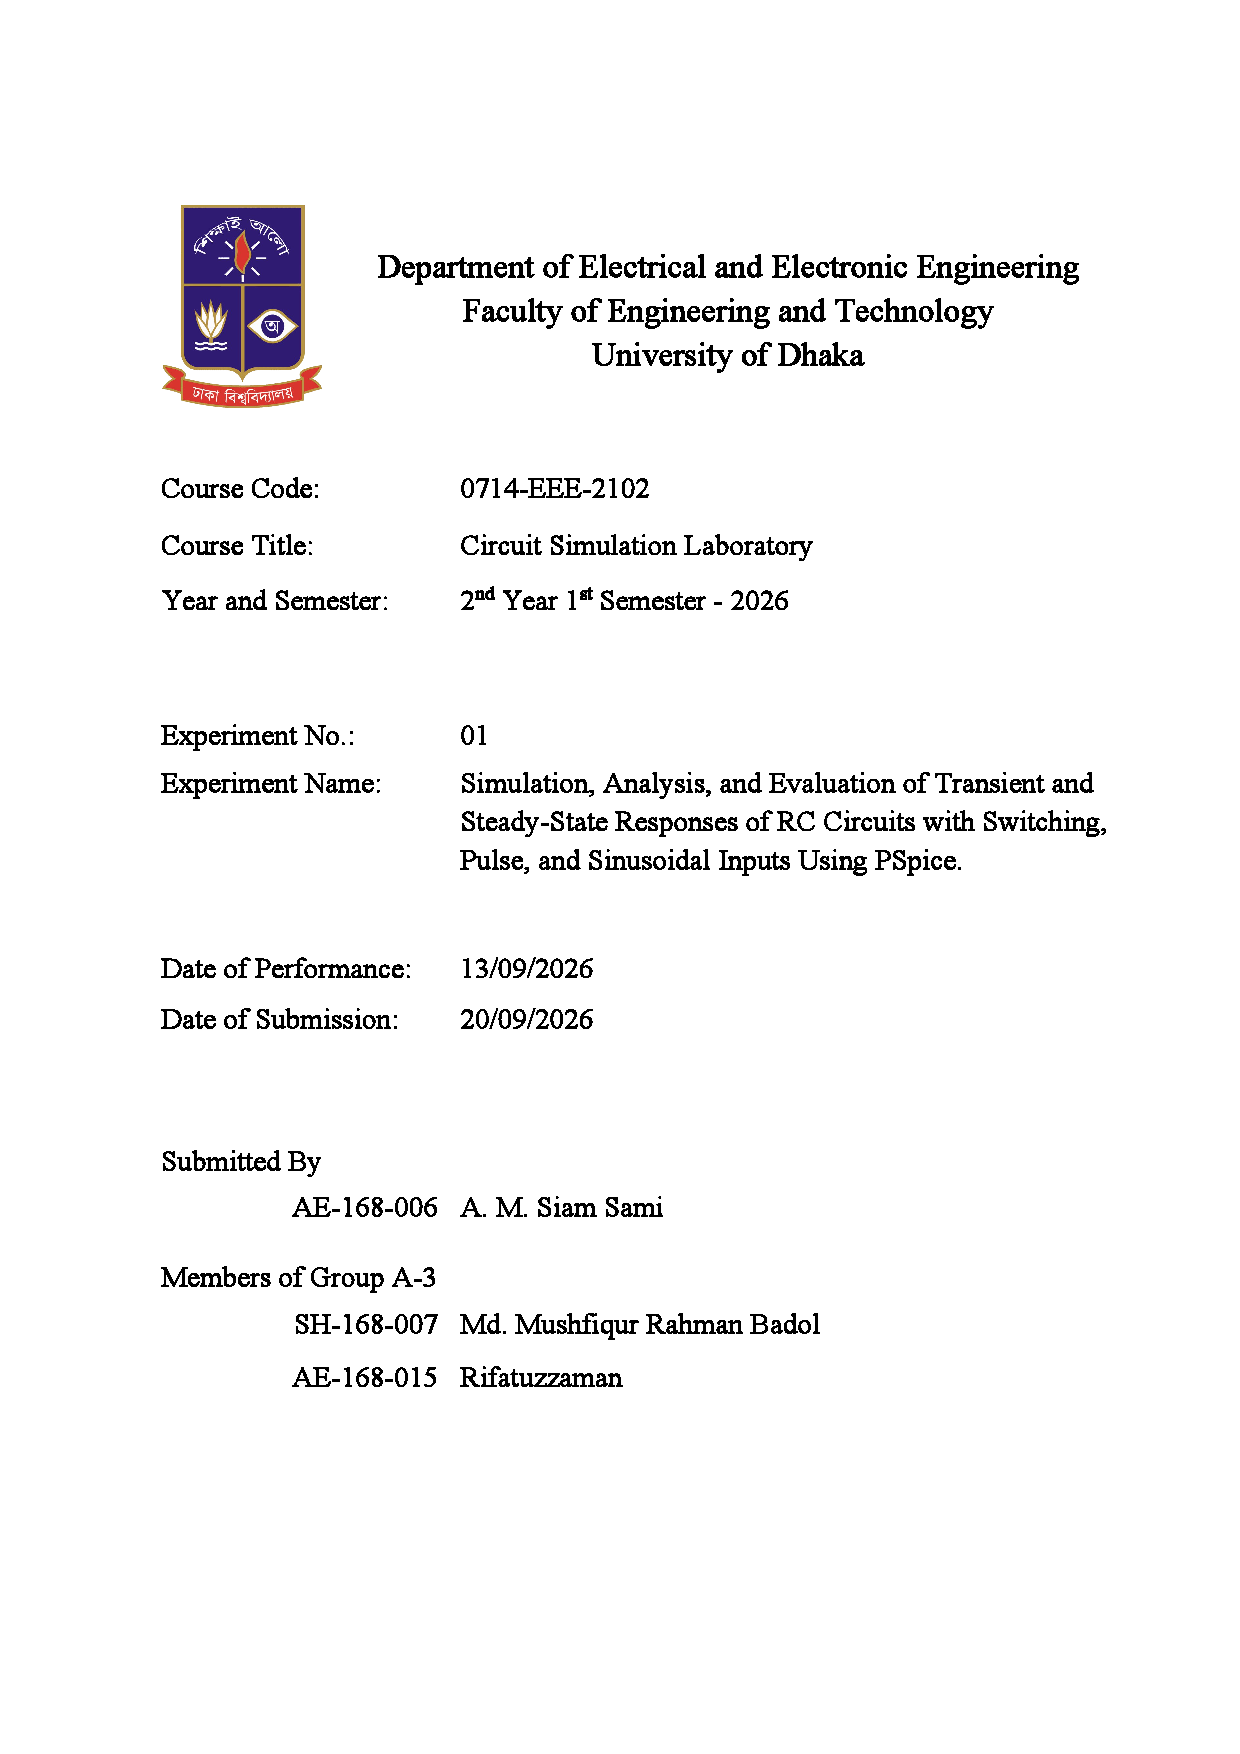
\includepdf[]{Cover_Page.pdf}
	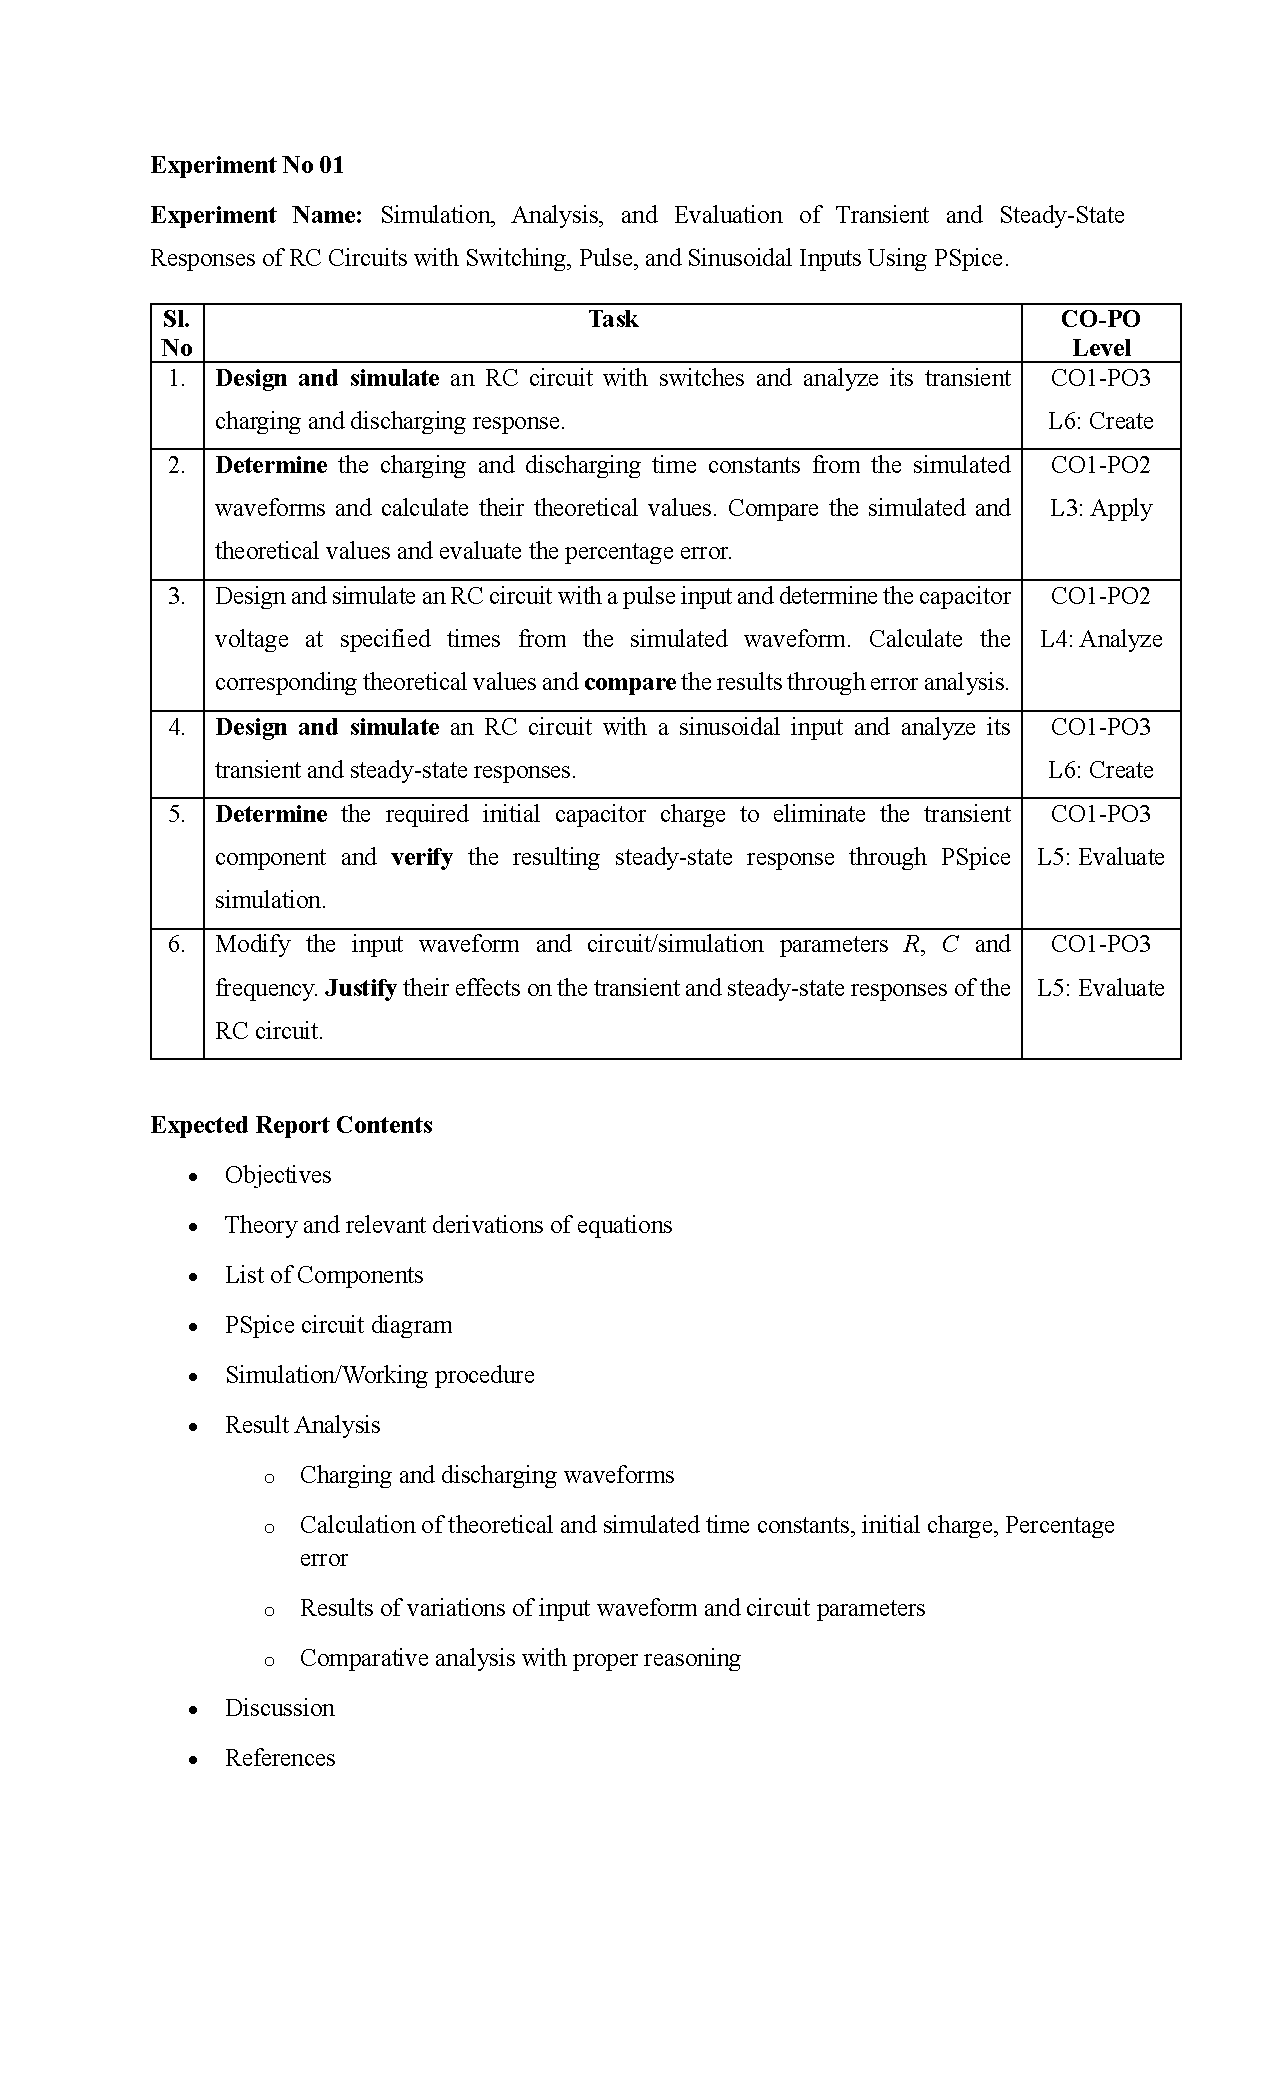
\includepdf[]{2nd_page.pdf}
	\pagenumbering{arabic}
	
	% =====================================================================
	% HEADER BLOCK
	% =====================================================================
	\begin{center}
		{\fontsize{14}{18}\selectfont\bfseries Experiment No. \expnumber}\\[4pt]
		{\fontsize{14}{18}\selectfont\bfseries Name of the Experiment: Simulation, Analysis, and
			Evaluation of Transient and Steady-State Responses of RC Circuits
			with Switching, Pulse, and Sinusoidal Inputs Using PSpice}
	\end{center}
	\vspace{6pt}
	
	% =====================================================================
	\section{Objective}
	% =====================================================================
	\begin{enumerate}[label=\roman*., leftmargin=2.5em]
		\item To design and simulate RC circuits driven by switched DC,
		pulse, and sinusoidal sources using PSpice.
		\item To analyze the transient charging and discharging responses and
		to determine the simulated time constants, comparing them with
		the theoretical values through percentage-error analysis.
		\item To determine the initial capacitor charge required to
		eliminate the transient component of the sinusoidal response,
		and to verify the resulting steady-state response by
		simulation.
		\item To investigate the effects of varying the input waveform and
		the circuit parameters ($R$, $C$, and frequency) on the
		transient and steady-state responses of the RC circuit.
	\end{enumerate}
	
	% =====================================================================
	\section{Theory}
	\label{sec:theory}
	% =====================================================================
	An RC circuit contains a resistor $R$ in series with a capacitor $C$
	and is the simplest circuit that exhibits a \emph{transient response}:
	whenever a source is suddenly connected, disconnected, or changed, the
	capacitor voltage cannot jump instantaneously because the charge on
	its plates, and hence the energy $\tfrac{1}{2}C\symup{v}_{\mathit{C}}^2$ stored in its
	electric field, can only change through a finite current.  The
	capacitor voltage therefore relaxes continuously from its initial
	value toward the new steady value demanded by the source, over a time
	set by the circuit itself.  This behavior is governed by a first-order
	differential equation, so every response in this experiment is a
	decaying exponential (or an exponential plus a sinusoid) whose
	characteristic time is the \emph{time constant} $\tau = RC$
	\cite{sadiku}, \cite{boylestad}.
	
	
	Fig.~\ref{fig:general-rc} shows the general series RC circuit,
	with the output voltage measured across the capacitor.
	
	\begin{figure}[H]
		\centering
		\begin{circuitikz}
			\draw (0,0) node[ground] {}
			to[V,invert,l=$\symup{v}_{\mathit{s}}(t)$] (0,3)
			to[R,l=$R$,i>^=$i(t)$] (5,3)
			to[C] (5,0)
			-- (0,0);
			\draw (5,3) to[short,*-o] (6,3);
			\draw (5,0) to[short,*-o] (6,0);
			\node at (6,2.6) {$+$};
			\node at (6,0.4) {$-$};
			\node at (4.1,1.5) {$C$};
			\node at (6.5,1.5) {$\symup{v}_{\mathit{C}}(t)$};
		\end{circuitikz}
		\caption{General series RC circuit with source voltage $\symup{v}_{\mathit{s}}(t)$,
			current $i(t)$, and capacitor voltage $\symup{v}_{\mathit{C}}(t)$; $\tau=RC$.}
		\label{fig:general-rc}
	\end{figure}
	
	\paragraph{Natural (source-free) response.}
	When a charged capacitor is left to discharge through a resistor,
	Kirchhoff's current law at the top node gives $\symup{i}_{\mathit{C}} + \symup{i}_{\mathit{R}} = 0$ with
	$\symup{i}_{\mathit{C}} = C\,d\symup{v}_{\mathit{C}}/dt$ and $\symup{i}_{\mathit{R}} = \symup{v}_{\mathit{C}}/R$, hence
	\begin{equation}
		RC\,\frac{d\symup{v}_{\mathit{C}}}{dt} + \symup{v}_{\mathit{C}} = 0 .
		\label{eq:natural-ode}
	\end{equation}
	Separating variables, $\dfrac{d\symup{v}_{\mathit{C}}}{\symup{v}_{\mathit{C}}} = -\dfrac{dt}{RC}$, and
	integrating both sides yields
	$\ln \symup{v}_{\mathit{C}} = -t/RC + \ln A$, so that
	\begin{equation}
		\symup{v}_{\mathit{C}}(t) = \symup{V}_{0}\, e^{-t/\tau}, \qquad \tau \equiv RC,
		\label{eq:natural}
	\end{equation}
	where the constant $A$ has been fixed by the initial condition
	$\symup{v}_{\mathit{C}}(0) = \symup{V}_{0}$, itself set by the initial charge $\symup{Q}_{0} = C \symup{V}_{0}$.  The
	response is entirely due to the energy initially stored, so it is
	called the \emph{natural response} of the circuit \cite{sadiku}.
	Because the discharge current $i = \symup{v}_{\mathit{C}}/R$ shrinks as $\symup{v}_{\mathit{C}}$ falls, the
	decay is fast at first and progressively slower: the voltage retains
	its polarity while the current direction reverses relative to the
	charging phase \cite{boylestad}.
	
	\paragraph{Time constant.}
	From Eq.~\eqref{eq:natural}, at $t = \tau$ the capacitor voltage has
	fallen to $\symup{V}_{0}/e \approx 0.368\,\symup{V}_{0}$ (36.8\,\% of its initial value);
	during charging it reaches $1 - 1/e \approx 0.632$ (63.2\,\%) of its
	final value.  This gives the practical measurement rule used
	throughout this experiment: the time constant is the interval from the
	switching instant to the 36.8\,\% (discharging) or 63.2\,\%
	(charging) point of the waveform \cite{boylestad}.  After $5\tau$ the
	exponential factor is $e^{-5} \approx 0.0067$, i.e.\ the response is
	within 0.7\,\% of its final value, which is conventionally regarded
	as complete settling \cite{sadiku}.  A small $\tau$ (small $R$, small
	$C$) means quick energy exchange and a fast response; a large $\tau$
	means slow relaxation.
	
	\paragraph{Step response (charging).}
	When a DC source $\symup{V}_{\mathit{s}}$ is suddenly applied to a series RC circuit
	with an arbitrary initial voltage $\symup{V}_{0}$, Kirchhoff's voltage law gives
	\begin{equation}
		RC\,\frac{d\symup{v}_{\mathit{C}}}{dt} + \symup{v}_{\mathit{C}} = \symup{V}_{\mathit{s}} .
		\label{eq:step-ode}
	\end{equation}
	Separating variables and integrating exactly as for
	Eq.~\eqref{eq:natural-ode},
	$\ln\!\left[\dfrac{\symup{v}_{\mathit{C}} - \symup{V}_{\mathit{s}}}{\symup{V}_{0} - \symup{V}_{\mathit{s}}}\right] = -t/\tau$, gives the
	\emph{complete response}
	\begin{equation}
		\symup{v}_{\mathit{C}}(t) = \symup{V}_{\mathit{s}} + (\symup{V}_{0} - \symup{V}_{\mathit{s}})\, e^{-t/\tau}.
		\label{eq:step}
	\end{equation}
	Equation~\eqref{eq:step} is the sum of a \emph{forced}
	(steady-state) part $\symup{V}_{\mathit{s}}$ and a \emph{natural} (transient) part
	$(\symup{V}_{0} - \symup{V}_{\mathit{s}})e^{-t/\tau}$; the transient exists only because the
	initial condition differs from the forced value \cite{sadiku}.  For an
	initially uncharged capacitor ($\symup{V}_{0} = 0$),
	\begin{equation}
		\symup{v}_{\mathit{C}}(t) = \symup{V}_{\mathit{s}}\left(1 - e^{-t/\tau}\right),
		\label{eq:charging}
	\end{equation}
	the familiar rising exponential: charge is deposited very rapidly at
	first (the full source voltage appears across $R$) and ever more
	slowly as $\symup{v}_{\mathit{C}}$ approaches $\symup{V}_{\mathit{s}}$ and the driving difference
	$\symup{v}_{\mathit{s}} - \symup{v}_{\mathit{C}}$ collapses \cite{boylestad}.  If the circuit contains
	several resistors, $\tau$ is computed with the Th\'evenin resistance
	seen at the capacitor terminals \cite{sadiku}.
	
	\paragraph{Pulse input.}
	A rectangular pulse of amplitude $\symup{V}_{\mathit{m}}$, width $\symup{T}_{\mathit{on}}$, and period $T$
	alternately connects the capacitor to $\symup{V}_{\mathit{m}}$ and to zero.  Each
	interval is a step response described by Eq.~\eqref{eq:step}:
	\begin{equation}
		\symup{v}_{\mathit{C}}(t) =
		\begin{cases}
			\symup{V}_{\mathit{m}}\left(1 - e^{-t/\tau}\right), & 0 \le t \le \symup{T}_{\mathit{on}}, \\[4pt]
			\symup{V}_{\mathit{m}}\left(1 - e^{-\symup{T}_{\mathit{on}}/\tau}\right) e^{-(t - \symup{T}_{\mathit{on}})/\tau},
			& \symup{T}_{\mathit{on}} < t \le T,
		\end{cases}
		\label{eq:pulse}
	\end{equation}
	and later cycles repeat from whatever voltage the capacitor has
	reached, using Eq.~\eqref{eq:step} with that value as $\symup{V}_{0}$.  If
	$\symup{T}_{\mathit{on}} \gg \tau$ (in practice $\ge 5\tau$) the capacitor fully
	charges and discharges within every cycle; if $\symup{T}_{\mathit{on}} \lesssim \tau$
	it never reaches the pulse amplitude.
	
	\paragraph{Sinusoidal input and phasor steady state.}
	For the sinusoid $\symup{v}_{\mathit{s}}(t) = \symup{V}_{\mathit{m}} \sin(\omega t + \phi)$, where the
	angular frequency $\omega = 2\pi f$ is set by the source frequency $f$
	in hertz, the steady state can be found with phasors.  The capacitor voltage--current
	relation $i = C\,dv/dt$ transforms to the phasor relation
	$I = j\omega C V$, i.e.\ the capacitor presents the impedance
	\begin{equation}
		\symup{Z}_{\mathit{C}} = \frac{V}{I} = \frac{1}{j\omega C},
		\label{eq:zc}
	\end{equation}
	so its voltage lags its current by $90^\circ$ \cite{sadiku}.  By
	phasor voltage division in the series RC circuit,
	\begin{equation}
		\mathbf{V}_{\mathit{C}} = \frac{\symup{Z}_{\mathit{C}}}{R + \symup{Z}_{\mathit{C}}}\,\mathbf{V}_{\mathit{s}}
		= \frac{1}{1 + j\omega\tau}\,\mathbf{V}_{\mathit{s}},
		\qquad \tau = RC .
		\label{eq:h}
	\end{equation}
	The transfer function $H(j\omega)$ of
	Eq.~\eqref{eq:h} has magnitude $1/\sqrt{1 + (\omega\tau)^2}$ and
	angle $-\tan^{-1}(\omega\tau)$, so the steady-state capacitor
	voltage is
	again sinusoidal, at the same frequency, with amplitude attenuated
	and phase lagging the source by
	\begin{equation}
		A = \frac{\symup{V}_{\mathit{m}}}{\sqrt{1 + (\omega\tau)^2}}, \qquad
		\theta = \tan^{-1}(\omega\tau),
		\label{eq:amp-lag}
	\end{equation}
	that is,
	\begin{equation}
		\symup{v}_{\mathit{C,SS}}(t) = A \sin(\omega t + \phi - \theta).
		\label{eq:ss}
	\end{equation}
	Equation~\eqref{eq:h} is the low-pass character of the RC circuit:
	well below the cutoff frequency $\symup{f}_{\mathit{c}} = 1/(2\pi\tau)$
	($\omega\tau \ll 1$) the capacitor follows the source almost
	undistorted, whereas well above it ($\omega\tau \gg 1$) the output is
	strongly attenuated and lags by nearly $90^\circ$ \cite{sadiku}.
	
	\paragraph{Transient elimination by initial charge.}
	With the source applied at $t = 0$ and an initial capacitor voltage
	$\symup{V}_{0}$, the complete response is the steady state plus a natural term:
	\begin{equation}
		\symup{v}_{\mathit{C}}(t) = \symup{v}_{\mathit{C,SS}}(t)
		+ \left[\symup{V}_{0} - \symup{v}_{\mathit{C,SS}}(0)\right] e^{-t/\tau}.
		\label{eq:complete-sine}
	\end{equation}
	The transient component vanishes if and only if the capacitor is
	pre-charged to exactly the steady-state value at the switching
	instant,
	\begin{equation}
		\symup{V}_{0} = \symup{v}_{\mathit{C,SS}}(0) = A \sin(\phi - \theta),
		\label{eq:ic-cond}
	\end{equation}
	corresponding to an initial charge
	\begin{equation}
		\symup{Q}_{0} = C\,\symup{V}_{0} = C\,A\sin(\phi - \theta).
		\label{eq:q0}
	\end{equation}
	This is the condition tested in Tasks 5 and 6d.  In the steady state
	the capacitor absorbs no net energy: with
	$\symup{v}_{\mathit{C,SS}} = A\sin(\omega t + \psi)$, its instantaneous power
	\begin{equation}
		\symup{p}_{\mathit{C}} = \symup{v}_{\mathit{C}}\,C\frac{d\symup{v}_{\mathit{C}}}{dt}
		= \tfrac{1}{2}\omega C A^{2}\sin\!\bigl(2(\omega t + \psi)\bigr)
		\label{eq:pcap}
	\end{equation}
	oscillates symmetrically about zero with a cycle mean of zero and a
	peak value of $\tfrac{1}{2}\omega C A^{2}$, as energy is alternately
	stored in the electric field and returned to the source.
	
	\paragraph{Comparison with theory.}
	Each measured quantity in this report is compared with its calculated
	value using the absolute percentage error
	\begin{equation}
		\% \text{ Error} =
		\left|\frac{\text{Theoretical} - \text{Simulated}}{\text{Theoretical}}\right|
		\times 100 ,
		\label{eq:perr}
	\end{equation}
	reported throughout the Result Analysis; where the theoretical value
	is itself zero, the absolute deviation is reported instead.
	
	\paragraph{Assumptions.}
	The analysis assumes ideal lumped components (no capacitor leakage or
	equivalent series resistance), a source resistance of zero, and
	switches that change state instantaneously.  In the simulations the
	switches are voltage-controlled elements with a small on-resistance
	($\symup{R}_{\mathit{on}} = \SI{1}{\milli\ohm}$) and a large but finite
	off-resistance ($\symup{R}_{\mathit{off}} = \SI{1}{\mega\ohm}$), and the initial
	capacitor voltage is set explicitly.  Because $\symup{R}_{\mathit{off}}$ is
	large but not infinite, an ``open'' switch still leaks a small
	current from the source rather than disconnecting it completely.
	Where this leakage path ($\symup{R}_{\mathit{off}}$) and the resistance
	$\symup{R}_{\mathit{d}}$ remaining between the capacitor node and the reference
	node form a voltage divider, the capacitor does not discharge fully
	to zero but relaxes to the small final value
	\begin{equation}
		\symup{V}_{\mathit{f}} = \symup{V}_{\mathit{s}}\,\frac{\symup{R}_{\mathit{d}}}{\symup{R}_{\mathit{off}} + \symup{R}_{\mathit{d}}},
		\label{eq:pedestal}
	\end{equation}
	so that Eq.~\eqref{eq:step} applies with $\symup{V}_{\mathit{s}} \to \symup{V}_{\mathit{f}}$ in
	place of the ideal zero final value.  This pedestal, and the
	corresponding hold-interval droop through the same leakage path, are
	quantified for each switching task in the Result Analysis and
	Discussion.
	
	\newpage
	
	% =====================================================================
	\section{List of Components}
	% =====================================================================
	Table~\ref{tab:components} lists the components and software used.
	
	\begin{table}[H]
		\centering
		\caption{List of components, instruments, and software (quantities
			count the distinct task schematics in which each value appears;
			Tasks 5 and 6d rerun the Task 4 and 6c schematics with an added
			initial condition)}
		\label{tab:components}
		\reporttablestyle
		\begin{tabularx}{\linewidth}{|c|P{4.2cm}|Y|c|}
			\hline
			\rowcolor{black!10}
			\textbf{Sl. No.} & \textbf{Component/Instrument} & \textbf{Specification/Value} & \textbf{Quantity} \\ \hline
			
			1 & Resistor & \SI{100}{\ohm}          & 2 \\ \hline
			2 & Resistor & \SI{500}{\ohm}          & 1 \\ \hline
			3 & Resistor & \SI{1}{\kilo\ohm}        & 3 \\ \hline
			4 & Resistor & \SI{1.8}{\kilo\ohm}      & 1 \\ \hline
			5 & Resistor & \SI{2}{\kilo\ohm}        & 1 \\ \hline
			6 & Resistor & \SI{3}{\kilo\ohm}        & 1 \\ \hline
			7 & Capacitor & \SI{1}{\micro\farad}   & 3 \\ \hline
			8 & Capacitor & \SI{5}{\micro\farad}   & 1 \\ \hline
			9 & Capacitor & \SI{50}{\micro\farad}  & 2 \\ \hline
			10 & DC voltage source & \SI{10}{\volt}; \SI{20}{\volt} & 2 \\ \hline
			11 & Pulse voltage source & $0$--\SI{5}{\volt}
			(Task 3: $5$/$\SI{10}{\milli\second}$;\;
			Task 6b: $25$/$\SI{50}{\milli\second}$) & 2 \\ \hline
			12 & Sinusoidal voltage source & \SI{10}{\volt},
			\SI{100}{\hertz}, $-70^\circ$;\; \SI{50}{\volt},
			\SI{200}{\hertz}, $-50^\circ$ & 2 \\ \hline
			13 & Simulation software & PSpice & 1 \\ \hline
			
		\end{tabularx}
	\end{table}
	
	% =====================================================================
	\section{Working Procedure}
	% =====================================================================
	The circuits were investigated using transient analysis in PSpice.
	The procedure below describes circuit construction, simulation setup,
	and waveform analysis for each task.
	
	\begin{enumerate}[label=\arabic*., leftmargin=2.5em, itemsep=6pt]
		\item \textbf{Prepare the schematic.}
		Open PSpice and create a new schematic.  Select
		\texttt{Draw} $\rightarrow$ \texttt{Get New Part...} to place
		components, and use \texttt{Draw} $\rightarrow$ \texttt{Wire}
		to connect them.  Rotate components using \texttt{Ctrl+R},
		double-click them to edit their properties, and connect the
		circuit reference node to \texttt{GND\_EARTH}.
		
		\item \textbf{Construct the switching circuit (Tasks 1 and 2).}
		Place a \texttt{VDC} source, \texttt{Sw\_tOpen} and
		\texttt{Sw\_tClose} switches, two resistors, and a capacitor.
		Connect them as shown in Fig.~\ref{fig:schematic-switching}.
		Set the source to \SI{10}{\volt}, R1 to \SI{1}{\kilo\ohm},
		R2 to \SI{1.8}{\kilo\ohm}, and C1 to
		\SI{1}{\micro\farad}.  Set U1 to open at
		\SI{6}{\milli\second} and U2 to close at
		\SI{7}{\milli\second}.
		
		\item \textbf{Simulate the switching response.}
		Use \texttt{Markers} $\rightarrow$ \texttt{Mark Voltage/Level}
		to measure the capacitor voltage.  Add a differential voltage
		marker using \textnormal{Mark Voltage Differential}, with the
		terminal locations and polarity shown in
		Fig.~\ref{fig:schematic-switching}.  Under
		\texttt{Analysis} $\rightarrow$ \texttt{Setup}, enable
		\texttt{Transient...} and open its settings.  Set both
		\texttt{Print Step} and \texttt{Step Ceiling} to
		\SI{1}{\micro\second}, and set \texttt{Final Time} to
		\SI{50}{\milli\second}.  Select
		\texttt{Skip initial transient solution}.  Save the schematic
		using \texttt{File} $\rightarrow$ \texttt{Save}, then run
		\texttt{Analysis} $\rightarrow$ \texttt{Simulate}.
		Observe the charging, holding, and discharging intervals.
		
		\item \textbf{Construct the pulse-driven circuit (Task 3).}
		Connect a \texttt{VPULSE} source, a \SI{1}{\kilo\ohm}
		resistor, and a \SI{1}{\micro\farad} capacitor as shown in
		Fig.~\ref{fig:schematic-pulse}.  Set the source properties to
		\texttt{V1=0}, \texttt{V2=5}, \texttt{TR=1n},
		\texttt{TF=1n}, \texttt{PW=5ms}, and \texttt{PER=10ms}.
		
		\item \textbf{Simulate the pulse response.}
		Place voltage-level markers at the source and capacitor
		terminals, and a differential marker across R1 with the
		polarity shown in Fig.~\ref{fig:schematic-pulse}.
		Set the transient \texttt{Final Time} to
		\SI{30}{\milli\second}, retain the \SI{1}{\micro\second}
		print step and step ceiling, and select
		\texttt{Skip initial transient solution}.  Save and simulate
		the circuit.  Observe the capacitor charging during each
		high-level interval and discharging during each low-level
		interval.
		
		\item \textbf{Construct the sinusoidally driven circuit (Task 4).}
		Connect a \texttt{VSIN} source, the two resistors, and C1 as
		shown in Fig.~\ref{fig:schematic-sine}.  Set the shunt
		resistor to \SI{500}{\ohm}, the series resistor to
		\SI{1}{\kilo\ohm}, and C1 to \SI{1}{\micro\farad}.
		Configure the source with \texttt{VOFF=0},
		\texttt{VAMPL=10}, \texttt{FREQ=100}, and
		\texttt{PHASE=-70}.
		
		\item \textbf{Simulate the sinusoidal response.}
		Place source-voltage, capacitor-voltage, and differential
		voltage markers as shown in Fig.~\ref{fig:schematic-sine}.
		Set \texttt{Final Time} to \SI{50}{\milli\second}, retain
		the \SI{1}{\micro\second} print step and step ceiling, and
		select \texttt{Skip initial transient solution}.
		Save and simulate the circuit.  Observe the initial transient
		and the subsequent steady-state waveform.  Plot the capacitor
		power using the product of its voltage and current, with the
		current reference directed into the positive-voltage terminal.
		
		\item \textbf{Apply the initial capacitor voltage (Task 5).}
		Retain the Task 4 circuit and simulation settings.
		Double-click C1 and set its initial-voltage property to
		\texttt{IC=-8.2748}.  This value is the calculated
		steady-state capacitor voltage at the switching instant,
		rounded to four decimal places.  Save and repeat the
		simulation, then compare the waveform with Task 4 to verify
		that the transient component is suppressed.
		
		\item \textbf{Investigate parameter variations (Tasks 6a--6c).}
		Repeat the corresponding switching, pulse, and sinusoidal
		simulations using
		Figs.~\ref{fig:schematic-task6a}, \ref{fig:schematic-task6b},
		\ref{fig:schematic-task6cd}
		and Table~\ref{tab:task6params}.  For Task 6a, use a
		\SI{20}{\volt} source, R1 = \SI{3}{\kilo\ohm},
		R2 = \SI{2}{\kilo\ohm}, and C1 = \SI{5}{\micro\farad};
		set the opening and closing times to \SI{75}{\milli\second}
		and \SI{76}{\milli\second}, respectively.
		For Task 6b, use R1 = \SI{100}{\ohm} and
		C1 = \SI{50}{\micro\farad}, with a pulse width of
		\SI{25}{\milli\second} and a period of
		\SI{50}{\milli\second}.  For Task 6c, use a
		\SI{50}{\volt}, \SI{200}{\hertz} sinusoidal source with
		phase $-50^\circ$, a \SI{100}{\ohm} series resistor,
		a \SI{1}{\kilo\ohm} shunt resistor, and a
		\SI{50}{\micro\farad} capacitor.  Use zero initial
		capacitor voltage for these runs and extend the simulation
		duration as needed to observe the slower responses.
		
		\item \textbf{Suppress the transient at the modified operating
			point (Task 6d).}
		Retain the Task 6c circuit and set the initial-voltage property
		of C1 to \texttt{IC=-5.935}.  Repeat the simulation and
		compare the capacitor voltage with Task 6c.  Also plot the
		capacitor power to observe the alternating storage and return
		of energy during steady-state operation.
		
		\item \textbf{Export waveforms and measure time constants.}
		Save the voltage and power plots and export the waveform data
		for analysis.  Record the capacitor voltages at the switching
		instants and pulse boundaries.  Use interpolation between
		adjacent samples to locate the 63.2\,\% charging and
		36.8\,\% discharging points, measured relative to the total
		voltage change.  Measure each time constant from the start of
		the corresponding charging or discharging interval.
		
		\item \textbf{Measure the transient and steady-state
			responses.}
		Read the charging and discharging voltages from the plotted
		waveform, allowing for the nonzero final voltage where the
		discharge does not settle to zero.  For the sinusoidal runs,
		measure the steady-state amplitude as the voltage of the highest
		peak of the capacitor waveform after the transient has decayed,
		and obtain the phase angle directly from the graph by measuring
		the time shift between corresponding points (zero crossings and
		peaks) of the source and capacitor waveforms.  Subtract the
		calculated steady-state response from the complete waveform to
		isolate the transient component, read its amplitude at $t = 0$,
		and read its time constant at the $36.8\,\%$ point of the
		residual.
		
		\item \textbf{Compare simulation and calculation.}
		Compare the measured time constants, waveform amplitudes,
		phase shifts, and initial capacitor charges with the values
		calculated in Section~\ref{sec:calc}.  Evaluate percentage
		errors using Eq.~\eqref{eq:perr}, and report absolute
		deviations when the theoretical value is zero.  Summarize the
		results in tables and discuss the effects of changing the
		source, component values, and initial capacitor voltage.
	\end{enumerate}
	
	% =====================================================================
	\section{Working Diagram}
	% =====================================================================
	The three circuit topologies used in the experiment are shown below as
	exported from the simulation schematics.  The Task 6 simulations reuse
	the same three topologies with the modified component and source
	values listed in Table~\ref{tab:task6params}; their updated schematics
	are also included below.
	
	\begin{figure}[H]
		\centering
		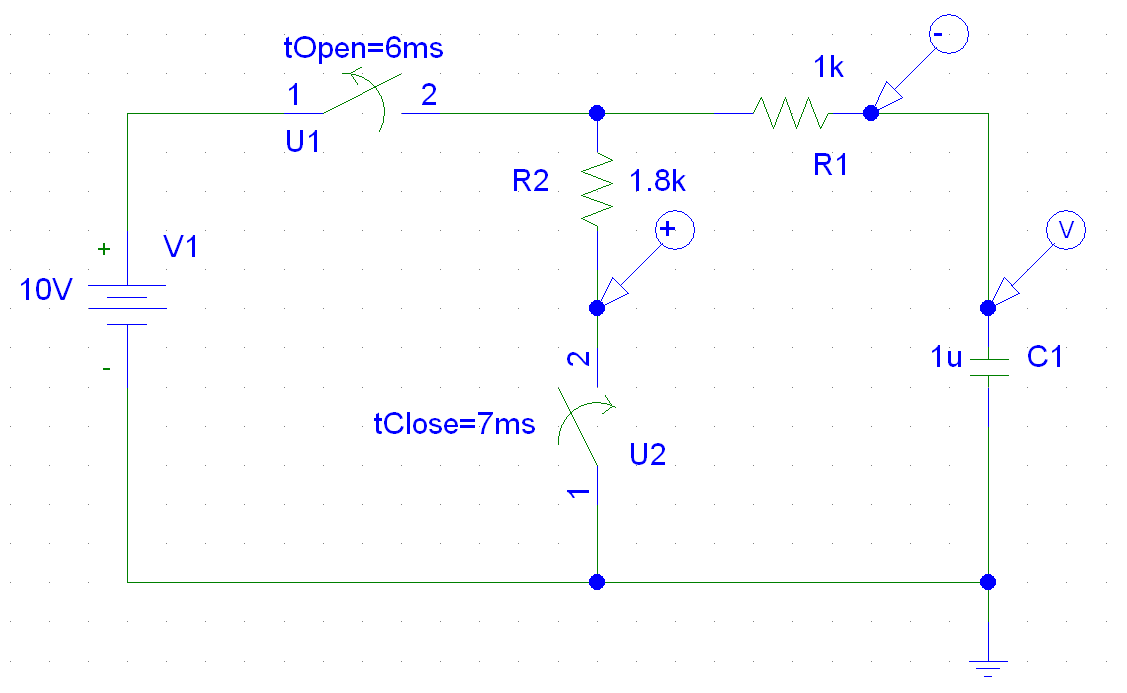
\includegraphics[width=0.85\textwidth,height=0.75\textheight,keepaspectratio]{circuit_task1,2.png}
		\caption{PSpice schematic of the switching RC circuit (Tasks 1 and 2): \SI{10}{\volt} DC source V1, \SI{1}{\kilo\ohm} charging
			resistor, \SI{1.8}{\kilo\ohm} discharge resistor, C1 =
			\SI{1}{\micro\farad}; U1 opens at $\symup{t}_{\mathit{open}} =
			\SI{6}{\milli\second}$ and U2 closes at $\symup{t}_{\mathit{close}} =
			\SI{7}{\milli\second}$.}
		\label{fig:schematic-switching}
	\end{figure}
	
	\begin{figure}[H]
		\centering
		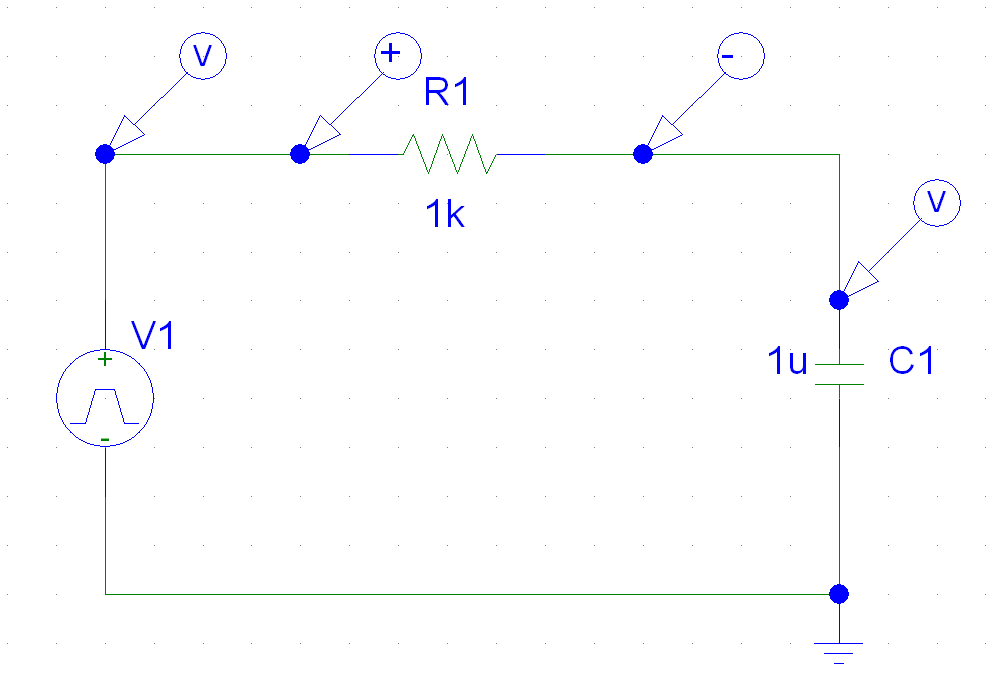
\includegraphics[width=0.8\textwidth,height=0.75\textheight,keepaspectratio]{circuit_task3.png}
		\caption{PSpice schematic of the pulse-driven RC circuit (Task 3):
			pulse source V1 (0--\SI{5}{\volt}, width \SI{5}{\milli\second},
			period \SI{10}{\milli\second}) in series with R1 =
			\SI{1}{\kilo\ohm} and C1 = \SI{1}{\micro\farad}.}
		\label{fig:schematic-pulse}
	\end{figure}
	
	\begin{figure}[H]
		\centering
		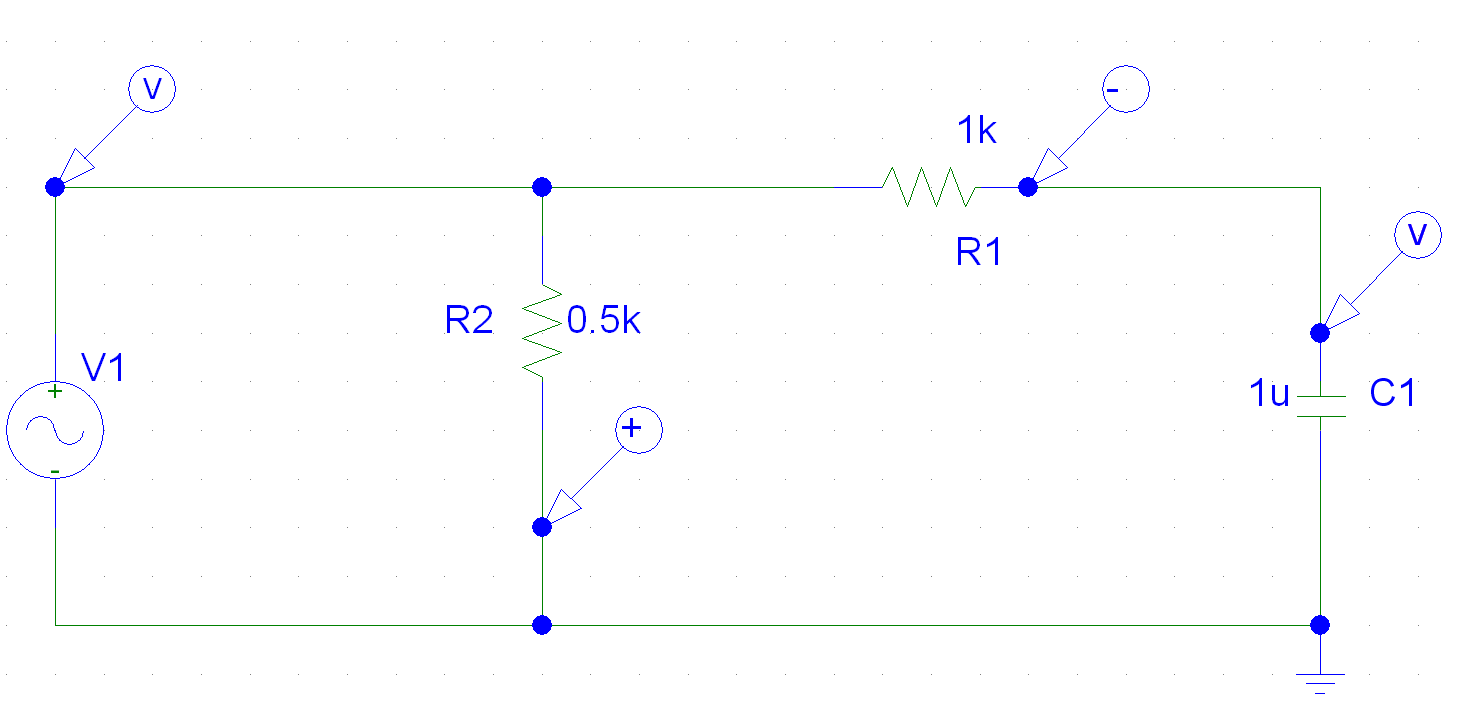
\includegraphics[width=0.85\textwidth,height=0.75\textheight,keepaspectratio]{circuit_task4,5.png}
		\caption{PSpice schematic of the sinusoidally driven RC circuit
			(Tasks 4 and 5): V1 = $10\sin(2\pi\cdot100 t -
			70^{\circ})$~V, \SI{500}{\ohm} shunt resistor across the source,
			\SI{1}{\kilo\ohm} series resistor, and C1 =
			\SI{1}{\micro\farad}; Task 5 adds the initial condition
			\texttt{IC = -8.2748}.}
		\label{fig:schematic-sine}
	\end{figure}
	
	\begin{figure}[H]
		\centering
		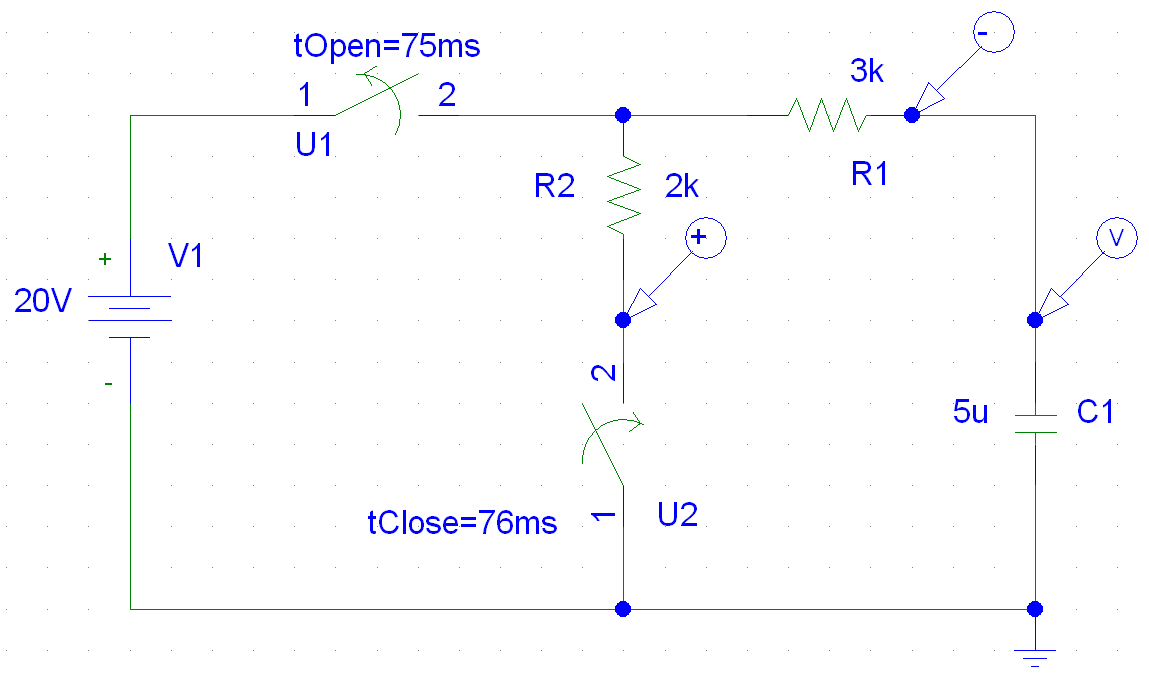
\includegraphics[width=0.85\textwidth,height=0.75\textheight,keepaspectratio]{circuit_task6a.png}
		\caption{PSpice schematic for Task 6a: \SI{20}{\volt} source,
			\SI{3}{\kilo\ohm} charging resistor, \SI{2}{\kilo\ohm}
			discharge resistor, and \SI{5}{\micro\farad} capacitor;
			U1 opens at \SI{75}{\milli\second} and U2 closes at
			\SI{76}{\milli\second}.}
		\label{fig:schematic-task6a}
	\end{figure}
	
	\begin{figure}[H]
		\centering
		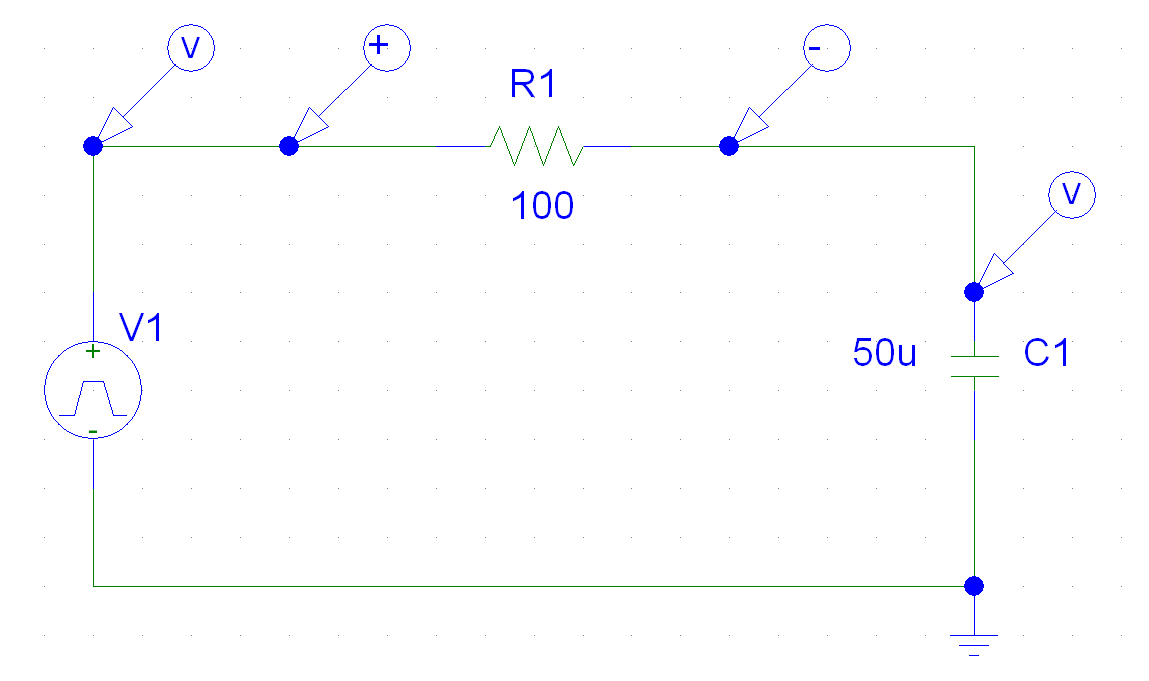
\includegraphics[width=0.8\textwidth,height=0.75\textheight,keepaspectratio]{circuit_task6b.png}
		\caption{PSpice schematic for Task 6b: pulse-driven RC circuit
			with R1 = \SI{100}{\ohm} and C1 = \SI{50}{\micro\farad}.}
		\label{fig:schematic-task6b}
	\end{figure}
	
	\begin{figure}[H]
		\centering
		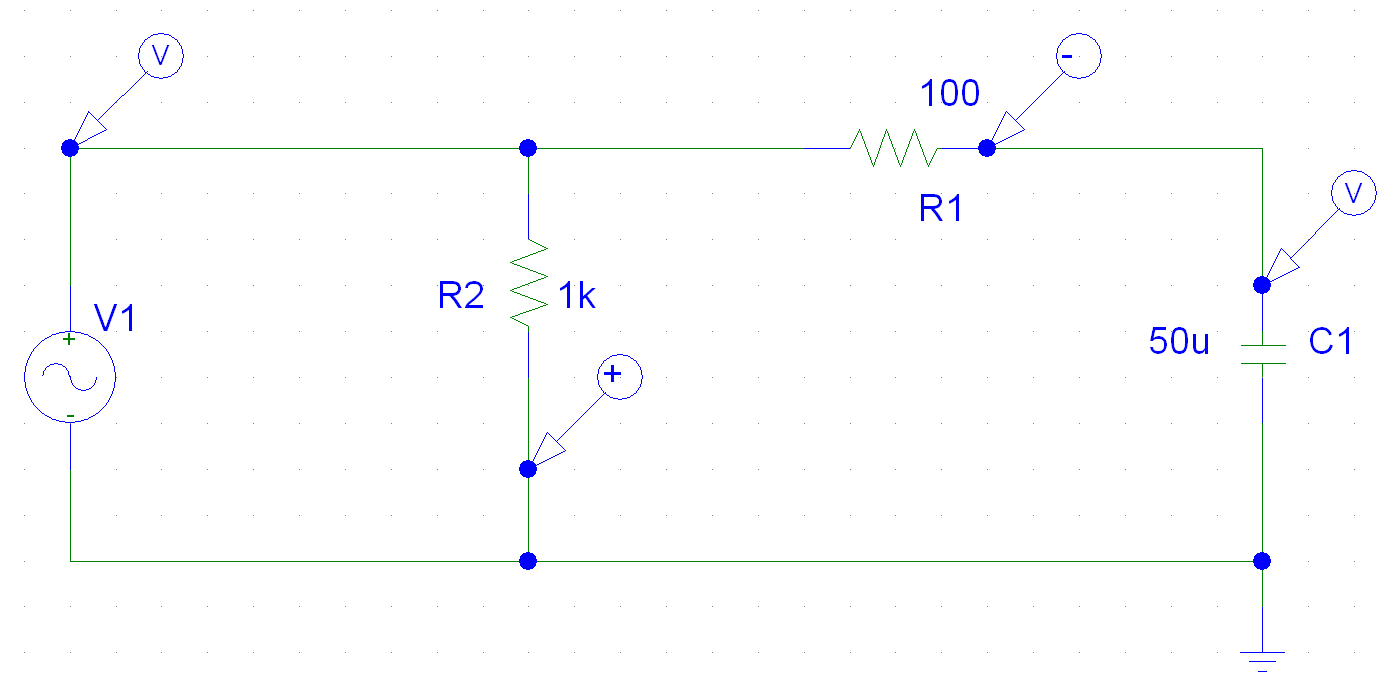
\includegraphics[width=0.85\textwidth,height=0.75\textheight,keepaspectratio]{circuit_task6c,d.png}
		\caption{PSpice schematic for Tasks 6c and 6d: sinusoidal source
			with a \SI{1}{\kilo\ohm} shunt resistor, \SI{100}{\ohm}
			series resistor, and \SI{50}{\micro\farad} capacitor;
			Task 6d applies the initial capacitor voltage
			\SI{-5.935}{\volt}.}
		\label{fig:schematic-task6cd}
	\end{figure}
	
	% =====================================================================
	\section{Calculation}
	\label{sec:calc}
	% =====================================================================
	\paragraph{Tasks 1: switching circuit.}
	$\symup{R}_{1} = \SI{1}{\kilo\ohm}$ denotes the charging resistor and
	$\symup{R}_{2} = \SI{1.8}{\kilo\ohm}$ the discharge resistor.  During charging
	($0 \le t \le \SI{6}{\milli\second}$) the source drives the capacitor
	through $\symup{R}_{1}$ alone, so $\tau = \symup{R}_{1}C$; after U2 closes the
	capacitor discharges through $\symup{R}_{1}$ and $\symup{R}_{2}$ in series.  With
	$C = \SI{1}{\micro\farad}$,
	\begin{align}
		\symup{\tau}_{\mathit{charge}} &= \symup{R}_{1} C
		= \left(1\times10^{3}\,\si{\ohm}\right)
		\left(1\times10^{-6}\,\si{\farad}\right)
		= \SI{1}{\milli\second}, \\
		\symup{\tau}_{\mathit{discharge}} &= (\symup{R}_{1} + \symup{R}_{2})\,C
		= \left(2.8\times10^{3}\,\si{\ohm}\right)
		\left(1\times10^{-6}\,\si{\farad}\right)
		= \SI{2.8}{\milli\second}.
	\end{align}
	The capacitor voltage when the source is disconnected at
	$t = \SI{6}{\milli\second}$ follows from Eq.~\eqref{eq:charging}:
	\begin{equation}
		\symup{v}_{\mathit{C}}(\SI{6}{\milli\second}) = 10\left(1 - e^{-6}\right)
		= 10 \times 0.997521 = \SI{9.9752}{\volt}.
	\end{equation}
	
	\paragraph{Task 3: pulse input.}
	Here $\tau = \symup{R}_{1} C = \SI{1}{\milli\second}$, and the pulse width
	($\SI{5}{\milli\second} = 5\tau$) allows essentially full charge and
	discharge every cycle.  From Eq.~\eqref{eq:pulse}, for example at
	$t = \SI{1}{\milli\second}$ (charging) and $t = \SI{6}{\milli\second}$
	(one $\tau$ into the discharge),
	\begin{align}
		\symup{v}_{\mathit{C}}(\SI{1}{\milli\second}) &= 5\left(1 - e^{-1}\right)
		= 5 \times 0.632121 = \SI{3.1606}{\volt}, \\
		\symup{v}_{\mathit{C}}(\SI{6}{\milli\second}) &= 5\left(1 - e^{-5}\right)e^{-1}
		= 4.9663 \times 0.367879 = \SI{1.8270}{\volt},
	\end{align}
	and the remaining instants of Table~\ref{tab:task3} follow the same
	way.
	
	\paragraph{Task 4: sinusoidal input.}
	The \SI{500}{\ohm} shunt resistor does not enter the calculation,
	because an ideal voltage source maintains its terminal voltage
	regardless of loading; the resistance seen by the capacitor is the
	series \SI{1}{\kilo\ohm} alone.  With $\omega = 2\pi f = 2\pi \times
	100 = \SI{628.32}{\radian\per\second}$ and
	$\tau = \SI{1}{\milli\second}$,
	\begin{equation}
		\omega\tau = 628.32 \times 10^{-3} = 0.6283,
	\end{equation}
	so Eq.~\eqref{eq:amp-lag} gives the steady-state amplitude and lag
	\begin{align}
		A &= \frac{10}{\sqrt{1 + 0.6283^2}}
		= \frac{10}{1.1810} = \SI{8.4673}{\volt},\\
		\theta &= \tan^{-1}(0.6283) = 32.14^{\circ}.
	\end{align}
	Since $A$ is by definition the peak value of the steady-state
	capacitor voltage, it is read from the simulated waveform as the
	voltage of the highest peak once the transient has decayed.  The lag
	$\theta$ appears on the same graph as a time shift $\Delta t$ between
	corresponding points of the source and capacitor waveforms, the two
	being related by
	\begin{equation}
		\theta = \omega\,\Delta t \ \text{(rad)}
		= 360^{\circ} f\,\Delta t \ \text{(deg)},
		\label{eq:phase-shift}
	\end{equation}
	so that at $f = \SI{100}{\hertz}$ (period $T = \SI{10}{\milli\second}$)
	the predicted lag corresponds to a measurable shift of
	\begin{equation}
		\Delta t = \frac{\theta}{360^{\circ}}\,T
		= \frac{32.14}{360} \times \SI{10}{\milli\second}
		= \SI{0.8928}{\milli\second}.
	\end{equation}
	The capacitor-voltage phase is $\phi - \theta = -70^\circ - 32.14^\circ
	= -102.14^\circ$, and the required initial voltage
	(Eq.~\eqref{eq:ic-cond}) is
	\begin{equation}
		\symup{V}_{0} = 8.4673\sin(-102.14^{\circ})
		= 8.4673 \times (-0.9776) = \SI{-8.278}{\volt},
	\end{equation}
	corresponding to an initial charge
	$\symup{Q}_{0} = C \symup{V}_{0} = (1\times10^{-6})(-8.278) =
	\SI{-8.278}{\micro\coulomb}$.  The circuit cutoff frequency is
	$\symup{f}_{\mathit{c}} = 1/(2\pi\tau) = \SI{159.2}{\hertz}$, so the
	\SI{100}{\hertz} excitation lies below cutoff
	($f/\symup{f}_{\mathit{c}} = 0.63$).  In the steady state the capacitor power
	oscillates with peak value (Eq.~\eqref{eq:pcap})
	\begin{equation}
		\symup{p}_{\mathit{C,peak}} = \tfrac{1}{2}\omega C A^{2}
		= \tfrac{1}{2}(628.32)\left(1\times10^{-6}\right)(8.4673)^2
		= \SI{22.5}{\milli\watt}
	\end{equation}
	and a cycle mean of zero.
	
	\paragraph{Task 5: transient elimination.}
	The applied initial condition is
	$\symup{V}_{\mathit{IC}} = \SI{-8.2748}{\volt}$ (the value of $\symup{V}_{0}$ above rounded to
	four decimal places).  The residual transient amplitude predicted by
	Eq.~\eqref{eq:complete-sine} is therefore
	\begin{equation}
		\left|\symup{V}_{\mathit{IC}} - \symup{V}_{0}\right| = \left|-8.2748 + 8.2779\right|
		= \SI{3.1}{\milli\volt},
	\end{equation}
	decaying with the same $\tau = \SI{1}{\milli\second}$; apart from
	this, the waveform should coincide with the theoretical steady state
	of Eq.~\eqref{eq:ss} from $t = 0$ onward.
	
	\paragraph{Task 6a: switching parameters changed.}
	With the charging resistor raised to \SI{3}{\kilo\ohm}, the
	discharge resistor to \SI{2}{\kilo\ohm}, and
	$C = \SI{5}{\micro\farad}$,
	\begin{align}
		\symup{\tau}_{\mathit{charge}} &= \left(3\times 10^{3}\right)\left(5\times 10^{-6}\right)
		= \SI{15}{\milli\second}, \\
		\symup{\tau}_{\mathit{discharge}} &= \left(5\times 10^{3}\right)\left(5\times 10^{-6}\right)
		= \SI{25}{\milli\second},
	\end{align}
	and U1 opens at exactly $5\symup{\tau}_{\mathit{charge}} =
	\SI{75}{\milli\second}$, at which point
	\begin{equation}
		\symup{v}_{\mathit{C}}(\SI{75}{\milli\second}) = 20\left(1 - e^{-5}\right)
		= \SI{19.8652}{\volt}.
	\end{equation}
	
	\paragraph{Task 6b: pulse parameters changed.}
	$\tau = \symup{R}_{1} C = (100)\left(50\times 10^{-6}\right) =
	\SI{5}{\milli\second}$, and both the \SI{25}{\milli\second} on and
	off intervals equal $5\tau$, so the capacitor nearly fully charges
	and discharges every cycle:
	\begin{align}
		\symup{v}_{\mathit{C}}(\SI{25}{\milli\second}) &= 5\left(1 - e^{-5}\right)
		= \SI{4.9663}{\volt},\\
		\symup{v}_{\mathit{C}}(\SI{50}{\milli\second}) &= 4.9663\, e^{-5} = \SI{0.0335}{\volt},
	\end{align}
	and the second cycle starts from \SI{0.0335}{\volt}:
	$\symup{v}_{\mathit{C}}(\SI{75}{\milli\second}) = 5 - (5 - 0.0335)e^{-5} =
	\SI{4.9665}{\volt}$, $\symup{v}_{\mathit{C}}(\SI{100}{\milli\second}) = \SI{0.0335}{\volt}$.
	
	\paragraph{Task 6c/d: sinusoid parameters changed.}
	With $f = \SI{200}{\hertz}$, series $R = \SI{100}{\ohm}$,
	$C = \SI{50}{\micro\farad}$ (the \SI{1}{\kilo\ohm} shunt does not
	enter, as in Task 4):
	\begin{equation}
		\omega\tau = 2\pi \times 200 \times (100)\left(50\times 10^{-6}\right)
		= 6.2832 \quad \left(= 2\pi\ \text{exactly}\right),
	\end{equation}
	\begin{align}
		A &= \frac{50}{\sqrt{1 + 6.2832^2}}
		= \frac{50}{6.3623} = \SI{7.8588}{\volt},\\
		\theta &= \tan^{-1}(6.2832) = 80.96^{\circ},
	\end{align}
	which by Eq.~\eqref{eq:phase-shift} corresponds, at
	$f = \SI{200}{\hertz}$ (period $T = \SI{5}{\milli\second}$), to a
	measurable time shift
	\begin{equation}
		\Delta t = \frac{\theta}{360^{\circ}}\,T
		= \frac{80.96}{360} \times \SI{5}{\milli\second}
		= \SI{1.124}{\milli\second}.
	\end{equation}
	The capacitor-voltage phase is $-50^\circ - 80.96^\circ =
	-130.96^\circ$, and
	\begin{equation}
		\symup{V}_{0} = 7.8588 \sin(-130.96^{\circ})
		= 7.8588 \times (-0.7552) = \SI{-5.935}{\volt},
	\end{equation}
	\begin{equation}
		\symup{Q}_{0} = C \symup{V}_{0} = \left(50\times 10^{-6}\right)(-5.935)
		= \SI{-296.75}{\micro\coulomb}.
	\end{equation}
	The cutoff is now $\symup{f}_{\mathit{c}} = 1/(2\pi\tau) = \SI{31.8}{\hertz}$, so the
	\SI{200}{\hertz} excitation is far above cutoff.
	
	% =====================================================================
	\section{Result Analysis}
	\label{sec:results}
	% =====================================================================
	All simulated quantities below were read directly from the exported
	waveforms by the cursor-and-interpolation procedure described in the
	Working Procedure (steps 11--13), and compared with theory using the
	percentage error of Eq.~\eqref{eq:perr}.  Voltages were read to the
	nearest millivolt (to \SI{0.1}{\milli\volt} where the display was
	zoomed on a small residual voltage), times to the nearest
	microsecond, and phase angles
	to the nearest $0.1^{\circ}$; the steady-state sinusoidal amplitudes,
	being read at the flat maximum of the waveform, are quoted to the
	nearest \SI{10}{\milli\volt}.  The percentage errors in the tables
	follow from these readings as displayed.  The waveform figures below
	show the exported simulation graphs.
	
	\subsection{Switch input (Task 1)}
	\begin{figure}[H]
		\centering
		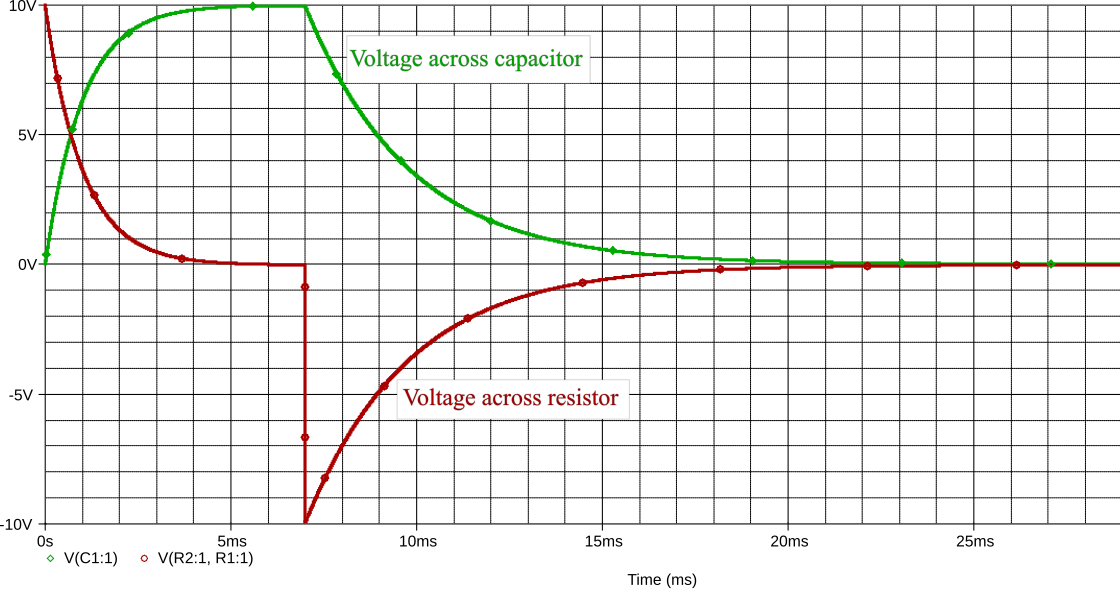
\includegraphics[width=\linewidth,height=0.4\textheight,keepaspectratio]{graph_task1,2.png}
		\caption{Simulated transient response of the switching RC circuit
			(Task 1): capacitor voltage charging during
			$0$--\SI{6}{\milli\second}, holding between
			\SI{6}{\milli\second} and \SI{7}{\milli\second}, and
			discharging after \SI{7}{\milli\second}.}
		\label{fig:task12}
	\end{figure}
	
	From Fig.~\ref{fig:task12}, the capacitor charges to
	\SI{9.975}{\volt} in \SI{6}{\milli\second} ($6\symup{\tau}_{\mathit{charge}}$), holds
	its voltage during the \SI{1}{\milli\second} interval in which both
	switches are open, and then decays through the
	\SI{2.8}{\kilo\ohm} path.  Table~\ref{tab:task12} compares the
	measured time constants and voltages with theory.
	
	\begin{table}[H]
		\centering
		\caption{Task 1: simulated vs.\ theoretical time constants
			and capacitor voltages}
		\label{tab:task12}
		\reporttablestyle
		\begin{tabularx}{\linewidth}{|Y|c|c|r|}
			\hline
			\rowcolor{black!10}
			\textbf{Quantity} & \textbf{Theoretical} & \textbf{Simulated} & \textbf{\% Error} \\ \hline
			
			$\symup{\tau}_{\mathit{charge}}$ (63.2\,\% crossing) & \SI{1.0000}{\milli\second} & \SI{0.999}{\milli\second} & $0.001$ \\ \hline
			$\symup{\tau}_{\mathit{discharge}}$ (36.8\,\% crossing) & \SI{2.8000}{\milli\second} & \SI{2.806}{\milli\second} & $0.214$ \\ \hline
			$\symup{v}_{\mathit{C}}$ at $t = \SI{6}{\milli\second}$ & \SI{9.9752}{\volt} & \SI{9.975}{\volt} & $0.002$ \\ \hline
			$\symup{v}_{\mathit{C}}$ at $t = \SI{7}{\milli\second}$ (hold) & \SI{9.9752}{\volt} & \SI{9.965}{\volt} & $0.102$ \\ \hline
			
		\end{tabularx}
	\end{table}
	
	The charging time constant matches theory almost exactly.  The
	$36.8\,\%$ crossing reads $\symup{\tau}_{\mathit{discharge}}$ $0.214\,\%$ high
	because the discharge never quite settles to zero: the open switch U1
	still feeds the loop through its \SI{1}{\mega\ohm} off-resistance, and
	by Eq.~\eqref{eq:pedestal} it leaves a final value
	$\symup{V}_{\mathit{s}} \symup{R}_{\mathit{d}}/(\symup{R}_{\mathit{off}}+\symup{R}_{\mathit{d}}) = 10 \times 1.8/(1000+1.8) =
	\SI{17.97}{\milli\volt}$ instead of zero. This off-resistance
	explains the \SI{10}{\milli\volt} hold-interval droop
	(Section~\ref{sec:discussion}).
	
	\subsection{Pulse input (Task 3)}
	\begin{figure}[H]
		\centering
		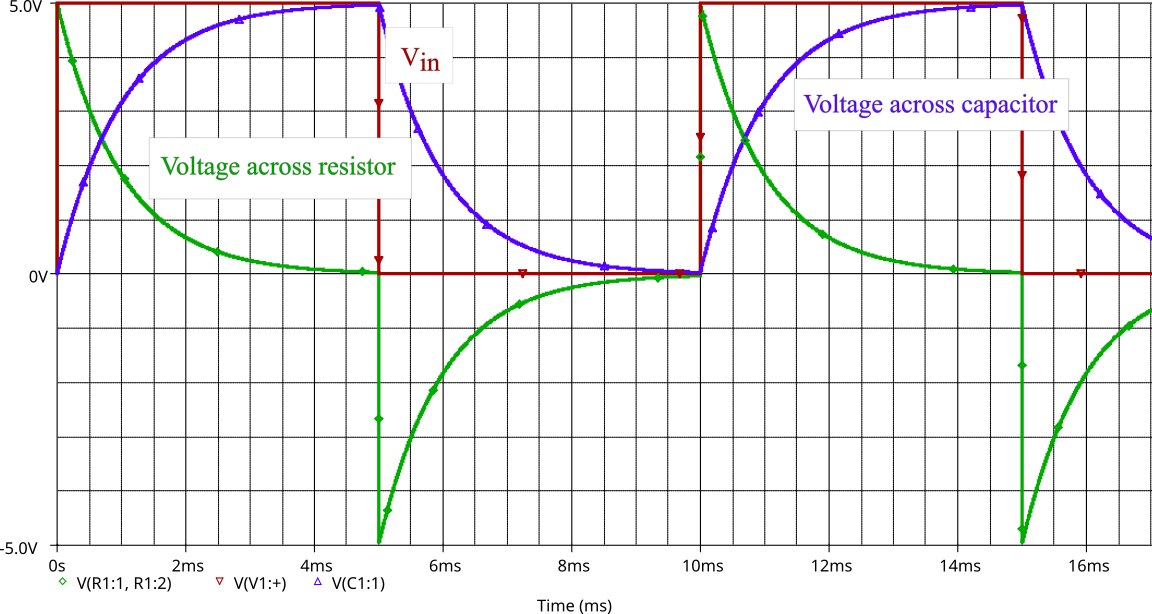
\includegraphics[width=\linewidth,height=0.4\textheight,keepaspectratio]{graph_task3.png}
		\caption{Simulated response of the RC circuit to the
			0--\SI{5}{\volt} pulse train (Task 3): the capacitor charges
			during each \SI{5}{\milli\second} on-interval and discharges
			during each \SI{5}{\milli\second} off-interval.}
		\label{fig:task3}
	\end{figure}
	
	Fig.~\ref{fig:task3} shows the exponential charge/discharge cycles
	predicted by Eq.~\eqref{eq:pulse}.  The simulated time constant, read
	at the 63.2\,\% crossing, is $\tau = \SI{1.000}{\milli\second}$,
	matching the calculated value to within the \SI{1}{\micro\second}
	reading resolution.  The capacitor voltage was read at every
	integer millisecond from $t = \SI{1}{\milli\second}$ to
	$t = \SI{10}{\milli\second}$, i.e.\ at every multiple of $\tau$
	across one complete pulse period (\SI{5}{\milli\second} on $+$
	\SI{5}{\milli\second} off); Table~\ref{tab:task3} lists the values.
	
	\begin{table}[H]
		\centering
		\caption{Task 3: capacitor voltage at specified times
			($\tau = \SI{1}{\milli\second}$, pulse $0$--\SI{5}{\volt},
			width \SI{5}{\milli\second}, period \SI{10}{\milli\second})}
		\label{tab:task3}
		\reporttablestyle
		\begin{tabularx}{\linewidth}{|Z|Z|Z|Z|}
			\hline
			\rowcolor{black!10}
			\textbf{Time (\si{\milli\second})} & \textbf{Theoretical $\symup{v}_{\mathit{C}}$ (\si{\volt})} & \textbf{Simulated $\symup{v}_{\mathit{C}}$ (\si{\volt})} & \textbf{\% Error} \\ \hline
			
			1 & 3.1606 & 3.161 & $0.013$ \\ \hline
			2 & 4.3233 & 4.323 & $0.007$ \\ \hline
			3 & 4.7511 & 4.751 & $0.002$ \\ \hline
			4 & 4.9084 & 4.908 & $0.008$ \\ \hline
			5 & 4.9663 & 4.966 & $0.006$ \\ \hline
			6 & 1.8270 & 1.827 & $0.000$ \\ \hline
			7 & 0.6721 & 0.6721 & $0.000$ \\ \hline
			8 & 0.2473 & 0.2472 & $0.040$ \\ \hline
			9 & 0.0910 & 0.0910 & $0.000$ \\ \hline
			10 & 0.0335 & 0.0335 & $0.000$ \\ \hline
			
		\end{tabularx}
	\end{table}
	
	Every sampled voltage in Table~\ref{tab:task3} agrees with
	Eq.~\eqref{eq:pulse} to better than $0.05\,\%$, consistent with the
	$5\tau$ settling rule.
	
	\subsection{Sinusoidal input, transient present (Task 4)}
	\begin{figure}[H]
		\centering
		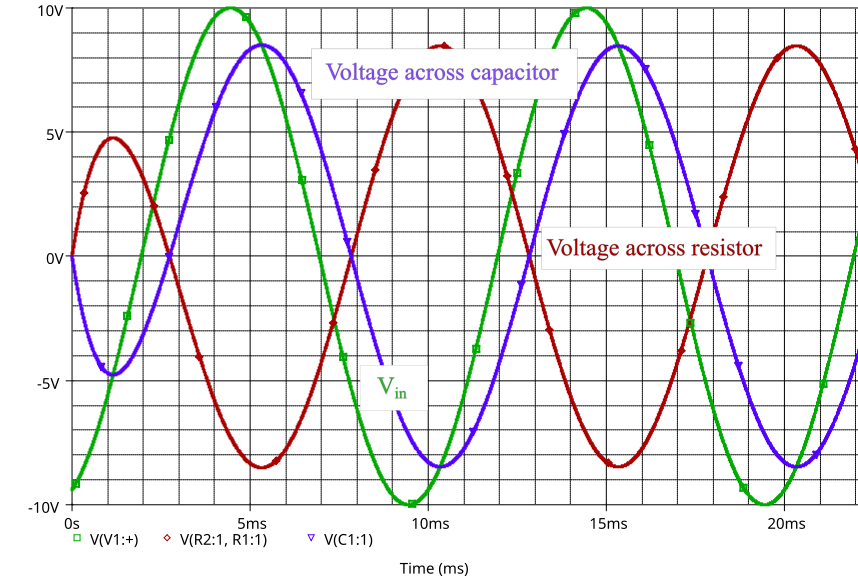
\includegraphics[width=\linewidth,height=0.4\textheight,keepaspectratio]{graph_task4.png}
		\caption{Simulated response of the RC circuit to
			$10\sin(2\pi\cdot100 t - 70^{\circ})$~\si{\volt} (Task 4): the capacitor
			voltage starts from zero and converges to the attenuated,
			phase-lagged steady-state sinusoid within about
			$5\tau = \SI{5}{\milli\second}$.}
		\label{fig:task4}
	\end{figure}
	
	The steady-state amplitude was obtained directly from
	Fig.~\ref{fig:task4} by measuring the voltage of the highest peak
	of the capacitor waveform after the transient had decayed, and the
	phase angle was measured directly from the same graph by measuring
	the time shift $\Delta t$ between corresponding points (zero
	crossings and peaks) of the source and capacitor waveforms and
	converting it with Eq.~\eqref{eq:phase-shift}.  The measured peak is
	\SI{8.47}{\volt}, and the measured shift,
	$\Delta t = \SI{0.893}{\milli\second}$ over the
	\SI{10}{\milli\second} period, gives
	$\theta = 360^{\circ}(100)(0.893\times10^{-3}) = 32.1^{\circ}$, so the
	capacitor-voltage phase is $-70^{\circ} - 32.1^{\circ} =
	-102.1^{\circ}$.  Subtracting the calculated steady state from the
	full waveform isolates the transient term, whose amplitude is read at
	$t = 0$ and whose time constant is read at the $36.8\,\%$ point of the
	residual; all are compared with the predictions of
	Section~\ref{sec:calc} (Table~\ref{tab:task4}).
	
	\begin{table}[H]
		\centering
		\caption{Task 4: sinusoidal steady-state and transient quantities}
		\label{tab:task4}
		\reporttablestyle
		\begin{tabularx}{\linewidth}{|Y|c|c|r|}
			\hline
			\rowcolor{black!10}
			\textbf{Quantity} & \textbf{Theoretical} & \textbf{Simulated} & \textbf{\% Error} \\ \hline
			
			Steady-state amplitude $A$ & \SI{8.4673}{\volt} & \SI{8.47}{\volt} & $0.032$ \\ \hline
			Phase of $\symup{v}_{\mathit{C}}$ & \SI{-102.142}{\degree} & \SI{-102.1}{\degree} & $0.041$ \\ \hline
			Phase lag $\theta$ & \SI{32.142}{\degree} & \SI{32.1}{\degree} & $0.131$ \\ \hline
			Transient amplitude & \SI{8.278}{\volt} & \SI{8.280}{\volt} & $0.024$ \\ \hline
			Transient time constant & \SI{1.0000}{\milli\second} & \SI{1.000}{\milli\second} & $0.000$ \\ \hline
			
		\end{tabularx}
	\end{table}
	
	The measured amplitude and phase match Eq.~\eqref{eq:amp-lag} to
	within the reading resolution ($0.03\,\%$ in amplitude,
	$0.05^{\circ}$ in phase): the output is attenuated to $84.7\,\%$ of
	the source amplitude and lags it by $32.1^\circ$, consistent with
	$f/\symup{f}_{\mathit{c}} = 0.63$.  The isolated transient,
	$8.280\,e^{-t/\tau}$~\si{\volt} with $\tau = \SI{1.000}{\milli\second}$,
	matches Eq.~\eqref{eq:complete-sine} for $\symup{V}_{0} = 0$.
	
	\begin{figure}[H]
		\centering
		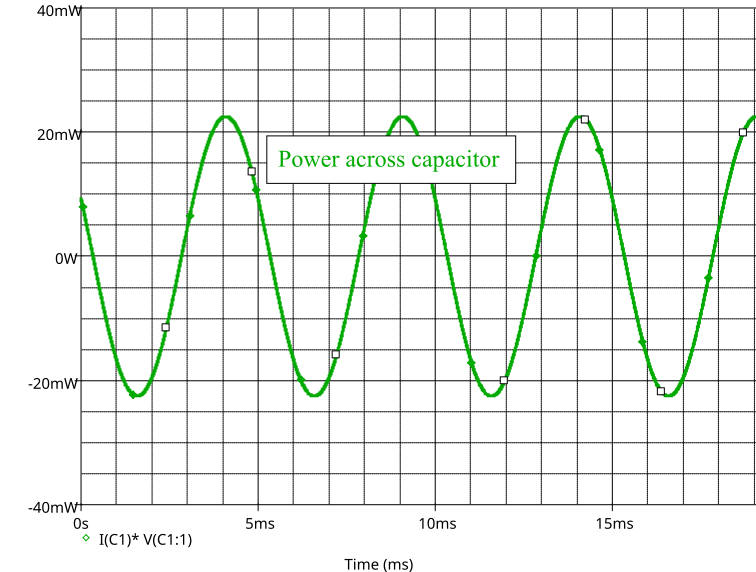
\includegraphics[width=\linewidth,height=0.4\textheight,keepaspectratio]{graph_task4_power.png}
		\caption{Instantaneous power of the capacitor for the Task 4 run:
			after the transient dies out the power oscillates symmetrically
			about zero with a peak of \SI{22.5}{\milli\watt}, indicating no
			net energy absorption in the steady state.}
		\label{fig:task4power}
	\end{figure}
	
	Fig.~\ref{fig:task4power} shows the corresponding capacitor power:
	once the transient has decayed, $\symup{p}_{\mathit{C}}(t)$ oscillates symmetrically
	about zero (measured peak $\pm\SI{22.5}{\milli\watt}$, cycle mean
	$\approx 0$), so the capacitor returns to the source exactly as much
	energy as it draws, the defining property of a reactive element in
	the steady state, and a direct check of Eq.~\eqref{eq:pcap}.
	
	\subsection{Transient elimination by initial charge (Task 5)}
	\begin{figure}[H]
		\centering
		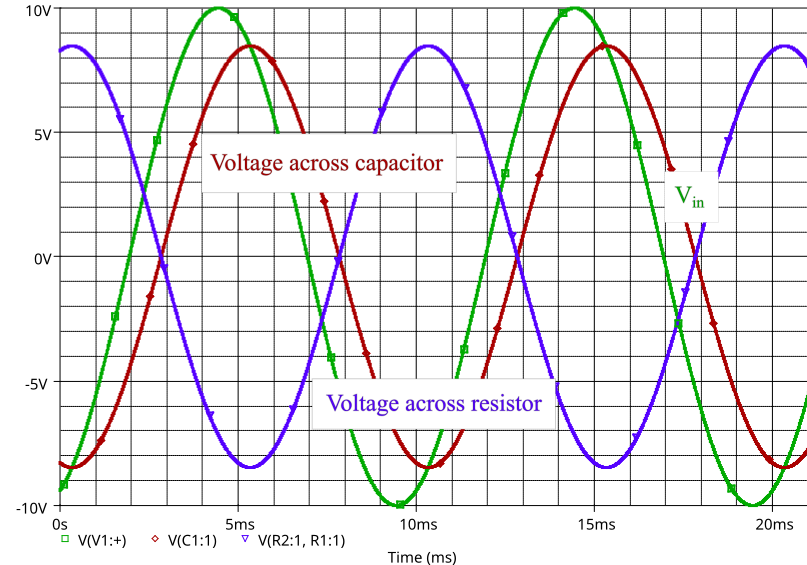
\includegraphics[width=\linewidth,height=0.4\textheight,keepaspectratio]{graph_task5.png}
		\caption{Task 5: with the initial condition
			\texttt{IC = -8.2748}, the capacitor voltage is a pure
			steady-state sinusoid from $t = 0$; no transient component is
			visible.}
		\label{fig:task5}
	\end{figure}
	
	With the capacitor pre-charged, the waveform of
	Fig.~\ref{fig:task5} is sinusoidal from the first instant: the
	natural term of Eq.~\eqref{eq:complete-sine} is absent.
	Table~\ref{tab:task5} compares the applied initial charge with the
	requirement of Eq.~\eqref{eq:ic-cond}.
	
	\begin{table}[H]
		\centering
		\caption{Task 5: initial capacitor charge required to eliminate the
			transient ($C = \SI{1}{\micro\farad}$)}
		\label{tab:task5}
		\reporttablestyle
		\begin{tabularx}{\linewidth}{|Y|c|c|r|}
			\hline
			\rowcolor{black!10}
			\textbf{Quantity} & \textbf{Theoretical} & \textbf{Simulated} & \textbf{\% Error} \\ \hline
			
			Required initial voltage $\symup{V}_{0}$ & \SI{-8.2779}{\volt} & \SI{-8.2748}{\volt} & $0.038$ \\ \hline
			Initial charge $\symup{Q}_{0} = C \symup{V}_{0}$ & \SI{-8.2779}{\micro\coulomb} & \SI{-8.2748}{\micro\coulomb} & $0.038$ \\ \hline
			Residual transient amplitude & \SI{3.1}{\milli\volt} & \SI{3.1}{\milli\volt} & --- \\ \hline
			
		\end{tabularx}
	\end{table}
	
	The simulated waveform coincides with the theoretical steady state
	of Eq.~\eqref{eq:ss} to within \SI{3.1}{\milli\volt} at $t = 0^{+}$,
	decaying with $\tau = \SI{1}{\milli\second}$. The residue expected
	simply from rounding $\symup{V}_{0}$ to four decimals (Eq.~\eqref{eq:complete-sine}).
	
	\subsection{Variation of input and circuit parameters (Task 6)}
	
	Table~\ref{tab:task6params} summarizes the parameter changes of the
	four Task 6 runs, using the updated schematics in
	Figs.~\ref{fig:schematic-task6a}, \ref{fig:schematic-task6b},
	\ref{fig:schematic-task6cd}.
	
	\begin{table}[H]
		\centering
		\caption{Task 6: parameter variations and their predicted effect}
		\label{tab:task6params}
		\reporttablestyle
		\begin{tabularx}{\linewidth}{|c|P{1.6cm}|Y|Y|}
			\hline
			\rowcolor{black!10}
			\textbf{Run} & \textbf{Based on} & \textbf{Changed parameters} & \textbf{Predicted effect} \\ \hline
			
			6a & Task 1/2 &
			$\symup{V}_{\mathit{s}}$: $10 \to \SI{20}{\volt}$; charging $R$: $\num{1} \to
			\SI{3}{\kilo\ohm}$; discharge $R$: $\num{1.8} \to
			\SI{2}{\kilo\ohm}$; $C$: $\num{1} \to
			\SI{5}{\micro\farad}$; switches $6/7 \to 75/76$~\si{\milli\second} &
			$\symup{\tau}_{\mathit{charge}}$: $1 \to \SI{15}{\milli\second}$;
			$\symup{\tau}_{\mathit{discharge}}$: $2.8 \to \SI{25}{\milli\second}$; opening
			at $5\symup{\tau}_{\mathit{charge}}$ \\ \hline
			6b & Task 3 &
			$R$: $\num{1} \to \SI{0.1}{\kilo\ohm}$; $C$: $\num{1} \to
			\SI{50}{\micro\farad}$; width $5 \to \SI{25}{\milli\second}$;
			period $10 \to \SI{50}{\milli\second}$ &
			$\tau$: $1 \to \SI{5}{\milli\second}$; on/off still $5\tau$
			each \\ \hline
			6c & Task 4 &
			$\symup{V}_{\mathit{m}}$: $10 \to \SI{50}{\volt}$; $f$: $100 \to
			\SI{200}{\hertz}$; series $R$: $\num{1} \to
			\SI{0.1}{\kilo\ohm}$; $C$: $\num{1} \to
			\SI{50}{\micro\farad}$ &
			$\omega\tau$: $0.63 \to 6.28$; $A$: $8.47 \to
			\SI{7.86}{\volt}$; $\theta$: $32.1^\circ \to 81.0^\circ$ \\ \hline
			6d & Task 6c &
			add \texttt{IC = -5.935} &
			transient eliminated; pure steady state from $t = 0$ \\ \hline
			
		\end{tabularx}
	\end{table}
	
	\paragraph{6a: switching circuit with larger $\tau$.}
	\begin{figure}[H]
		\centering
		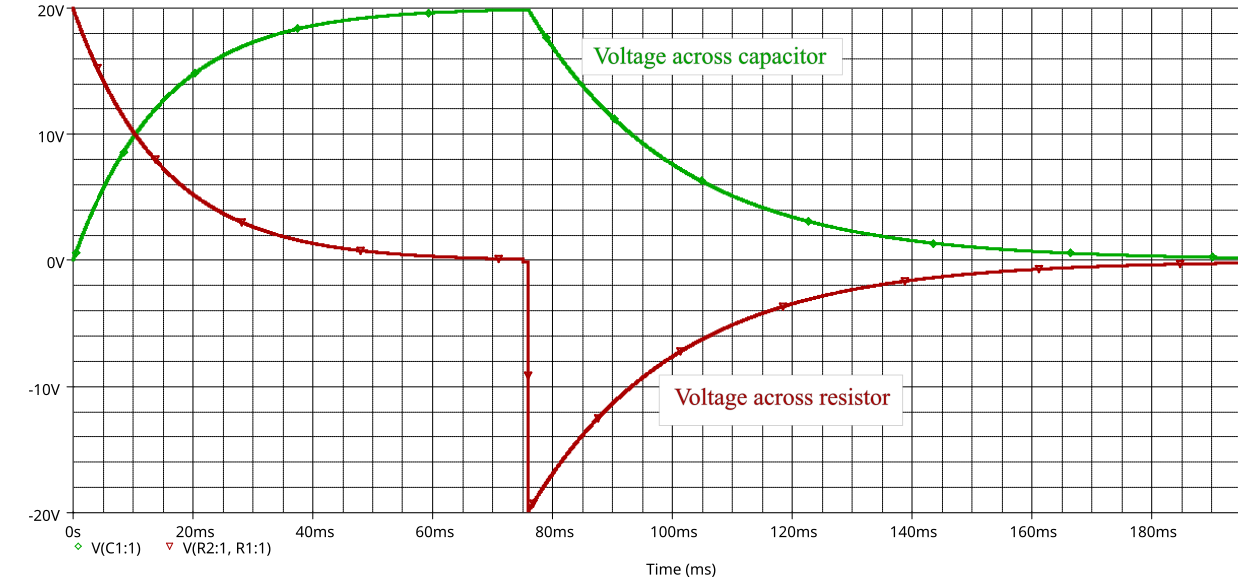
\includegraphics[width=\linewidth,height=0.4\textheight,keepaspectratio]{graph_task6a.png}
		\caption{Task 6a: response of the switching RC circuit with
			\SI{3}{\kilo\ohm} charging resistor, \SI{5}{\kilo\ohm} discharge
			path, $C = \SI{5}{\micro\farad}$, and \SI{20}{\volt} source:
			charging for \SI{75}{\milli\second} ($5\symup{\tau}_{\mathit{charge}}$), hold for
			\SI{1}{\milli\second}, discharging with
			$\symup{\tau}_{\mathit{discharge}} = \SI{25}{\milli\second}$.}
		\label{fig:task6a}
	\end{figure}
	
	\begin{table}[H]
		\centering
		\caption{Task 6a: simulated vs.\ theoretical time constants and
			voltages}
		\label{tab:task6a}
		\reporttablestyle
		\begin{tabularx}{\linewidth}{|Y|c|c|r|}
			\hline
			\rowcolor{black!10}
			\textbf{Quantity} & \textbf{Theoretical} & \textbf{Simulated} & \textbf{\% Error} \\ \hline
			
			$\symup{\tau}_{\mathit{charge}}$ (63.2\,\% crossing) & \SI{15.0000}{\milli\second} & \SI{14.999}{\milli\second} & $0.007$ \\ \hline
			$\symup{\tau}_{\mathit{discharge}}$ (36.8\,\% crossing) & \SI{25.0000}{\milli\second} & \SI{25.067}{\milli\second} & $0.268$ \\ \hline
			$\symup{v}_{\mathit{C}}$ at $t = \SI{75}{\milli\second}$ & \SI{19.8652}{\volt} & \SI{19.865}{\volt} & $0.001$ \\ \hline
			
		\end{tabularx}
	\end{table}
	
	The waveform of Fig.~\ref{fig:task6a} is a time-stretched version
	of the Task 1/2 response, with the same off-resistance pedestal of
	Eq.~\eqref{eq:pedestal} (here $20 \times 2/(1000+2) =
	\SI{39.92}{\milli\volt}$) biasing the discharge crossing reading
	(Table~\ref{tab:task6a}); The source disconnects at exactly $5\symup{\tau}_{\mathit{charge}}$, and
	the capacitor holds $99.33\,\%$ of \SI{20}{\volt} at that instant,
	in agreement with the $5\tau$ rule.
	
	\paragraph{6b: pulse circuit with larger $\tau$.}
	\begin{figure}[H]
		\centering
		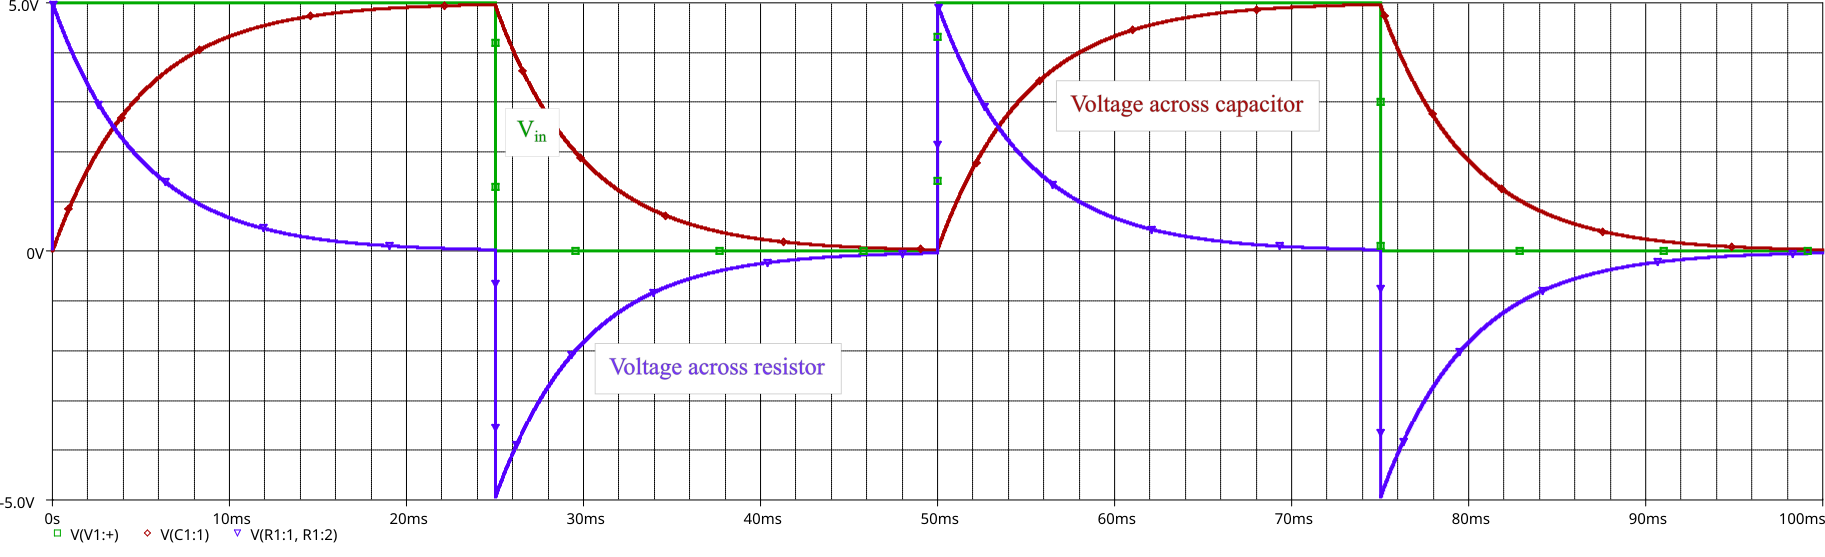
\includegraphics[width=\linewidth,height=0.4\textheight,keepaspectratio]{graph_task6b.png}
		\caption{Task 6b: response to the 0--\SI{5}{\volt} pulse train with
			$\tau = \SI{5}{\milli\second}$; each \SI{25}{\milli\second}
			half-cycle lasts $5\tau$, so the capacitor reaches
			$99.3\,\%$ of the pulse amplitude every cycle.}
		\label{fig:task6b}
	\end{figure}
	
	\begin{table}[H]
		\centering
		\caption{Task 6b: time constant and capacitor voltage at the
			cycle boundaries}
		\label{tab:task6b}
		\reporttablestyle
		\begin{tabularx}{\linewidth}{|Y|c|c|r|}
			\hline
			\rowcolor{black!10}
			\textbf{Quantity} & \textbf{Theoretical} & \textbf{Simulated} & \textbf{\% Error} \\ \hline
			
			$\tau$ (63.2\,\% crossing) & \SI{5.0000}{\milli\second} & \SI{5.000}{\milli\second} & $0.000$ \\ \hline
			$\symup{v}_{\mathit{C}}$ at $t = \SI{25}{\milli\second}$ & \SI{4.9663}{\volt} & \SI{4.966}{\volt} & $0.006$ \\ \hline
			$\symup{v}_{\mathit{C}}$ at $t = \SI{50}{\milli\second}$ & \SI{0.0335}{\volt} & \SI{0.0335}{\volt} & $0.000$ \\ \hline
			$\symup{v}_{\mathit{C}}$ at $t = \SI{75}{\milli\second}$ & \SI{4.9665}{\volt} & \SI{4.967}{\volt} & $0.010$ \\ \hline
			$\symup{v}_{\mathit{C}}$ at $t = \SI{100}{\milli\second}$ & \SI{0.0335}{\volt} & \SI{0.0335}{\volt} & $0.000$ \\ \hline
			
		\end{tabularx}
	\end{table}
	
	Despite the $25\times$ slower circuit ($\tau =
	\SI{5}{\milli\second}$ vs.\ \SI{1}{\milli\second}), the pulse width
	was enlarged by the same factor, so the waveform of
	Fig.~\ref{fig:task6b} retains the full-swing charge/discharge
	character of Task 3 (Table~\ref{tab:task6b}); only the small
	($0.7\,\%$) residue at each half-cycle boundary differs slightly
	between the first and second cycles, because the second discharge
	starts from the first cycle's residue.
	
	\paragraph{6c: sinusoid with increased frequency and
		attenuation.}
	\begin{figure}[H]
		\centering
		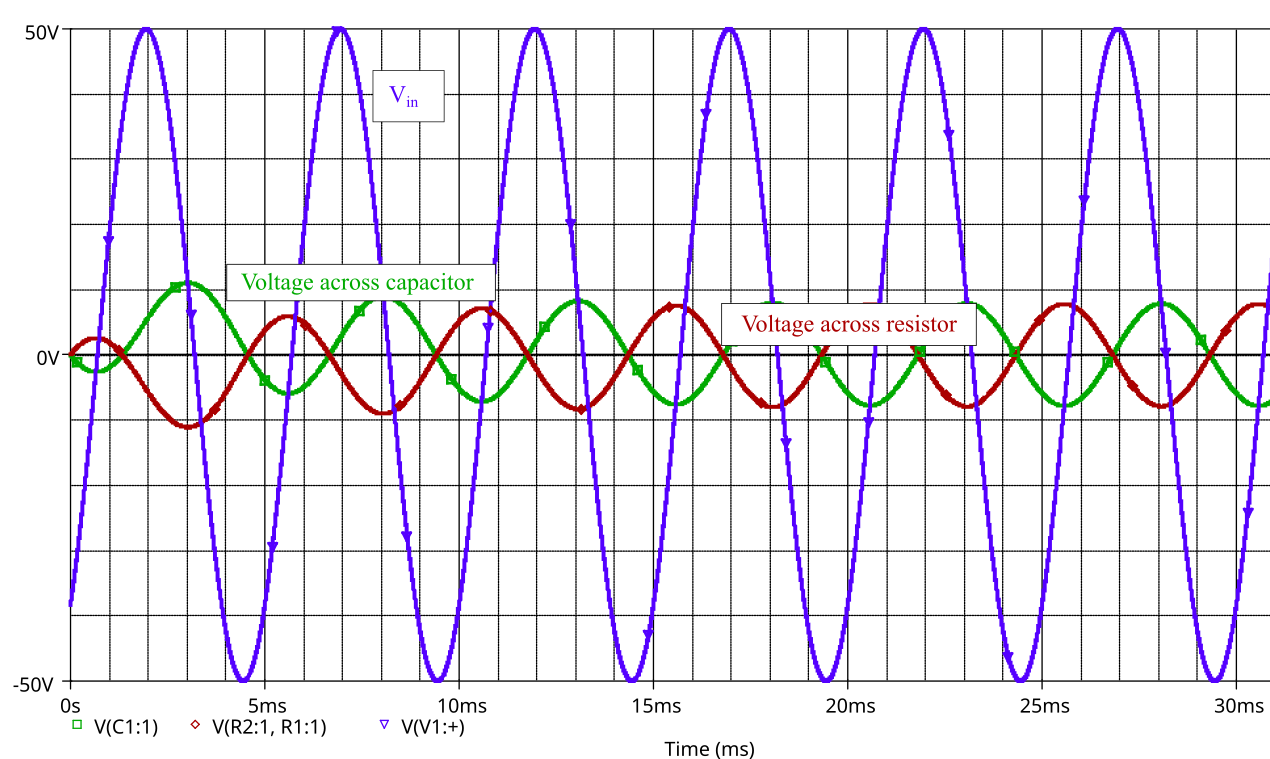
\includegraphics[width=\linewidth,height=0.4\textheight,keepaspectratio]{graph_task6c.png}
		\caption{Task 6c: response to
			$50\sin(2\pi\cdot200 t - 50^{\circ})$~\si{\volt} with $\tau =
			\SI{5}{\milli\second}$ ($\omega\tau = 2\pi$): the steady-state
			capacitor voltage is attenuated to \SI{7.86}{\volt} and lags the
			source by $81^\circ$; the \SI{5.935}{\volt} transient decays
			with $\tau = \SI{5}{\milli\second}$ and is still about
			\SI{0.1}{\volt} at $t = \SI{20}{\milli\second}$.}
		\label{fig:task6c}
	\end{figure}
	
	\begin{table}[H]
		\centering
		\caption{Task 6c: sinusoidal steady-state and transient quantities}
		\label{tab:task6c}
		\reporttablestyle
		\begin{tabularx}{\linewidth}{|Y|c|c|r|}
			\hline
			\rowcolor{black!10}
			\textbf{Quantity} & \textbf{Theoretical} & \textbf{Simulated} & \textbf{\% Error} \\ \hline
			
			Steady-state amplitude $A$ & \SI{7.8588}{\volt} & \SI{7.86}{\volt} & $0.015$ \\ \hline
			Phase of $\symup{v}_{\mathit{C}}$ & \SI{-130.957}{\degree} & \SI{-131.0}{\degree} & $0.033$ \\ \hline
			Phase lag $\theta$ & \SI{80.957}{\degree} & \SI{81.0}{\degree} & $0.053$ \\ \hline
			Transient amplitude & \SI{5.935}{\volt} & \SI{5.935}{\volt} & $0.000$ \\ \hline
			Transient time constant & \SI{5.0000}{\milli\second} & \SI{5.000}{\milli\second} & $0.000$ \\ \hline
			
		\end{tabularx}
	\end{table}
	
	Compared with Task 4, the excitation now lies far above cutoff
	($f/\symup{f}_{\mathit{c}} = 6.28$), so the same transfer function of
	Eq.~\eqref{eq:h} predicts (and the peak and time-shift measurements
	of Fig.~\ref{fig:task6c} confirm) strong attenuation (to $15.7\,\%$ of the
	\SI{50}{\volt} amplitude) and a lag approaching $90^\circ$
	(Table~\ref{tab:task6c}).  The highest peak of the steady portion
	reads \SI{7.86}{\volt}, and the measured shift $\Delta t =
	\SI{1.125}{\milli\second}$ over the \SI{5}{\milli\second} period gives
	$\theta = 81.0^{\circ}$ by Eq.~\eqref{eq:phase-shift}.  The isolated
	transient $5.935\,e^{-t/\tau}$~\si{\volt} matches the theoretical
	$-\symup{v}_{\mathit{C,SS}}(0)$ from Eq.~\eqref{eq:complete-sine}.
	
	\paragraph{6d: transient elimination at the new operating point.}
	\begin{figure}[H]
		\centering
		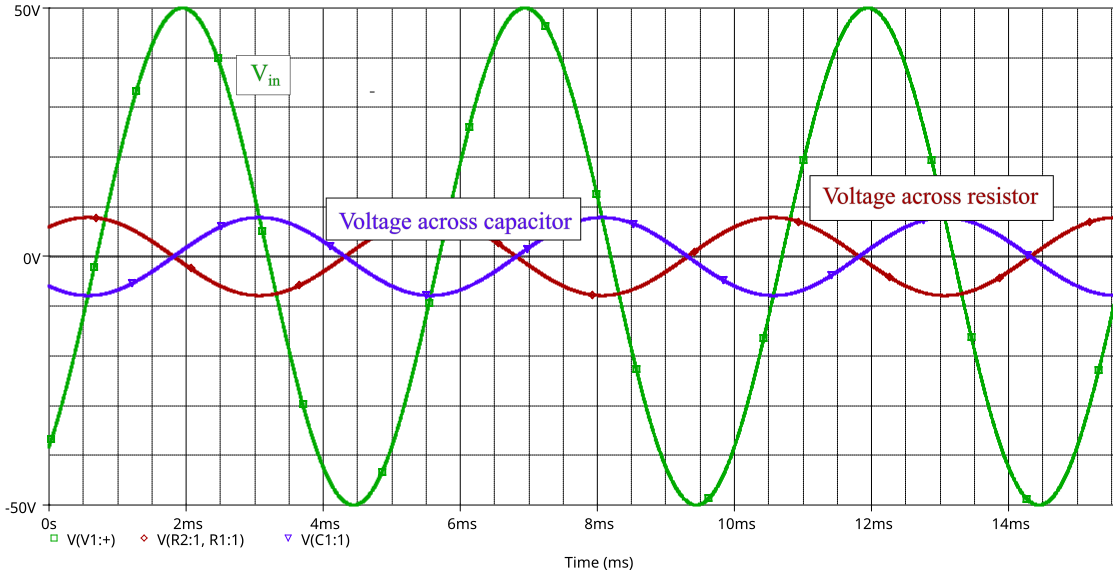
\includegraphics[width=\linewidth,height=0.4\textheight,keepaspectratio]{graph_task6d.png}
		\caption{Task 6d: with \texttt{.ic V(N002) = -5.935} the capacitor
			voltage is the pure steady-state sinusoid from $t = 0$; the
			transient of Fig.~\ref{fig:task6c} is absent.}
		\label{fig:task6d}
	\end{figure}
	
	\begin{table}[H]
		\centering
		\caption{Task 6d: initial charge required to eliminate the
			transient ($C = \SI{50}{\micro\farad}$)}
		\label{tab:task6d}
		\reporttablestyle
		\begin{tabularx}{\linewidth}{|Y|c|c|r|}
			\hline
			\rowcolor{black!10}
			\textbf{Quantity} & \textbf{Theoretical} & \textbf{Simulated} & \textbf{\% Error} \\ \hline
			
			Required initial voltage $\symup{V}_{0}$ & \SI{-5.9350}{\volt} & \SI{-5.9350}{\volt} & $0.000$ \\ \hline
			Initial charge $\symup{Q}_{0} = C \symup{V}_{0}$ & \SI{-296.75}{\micro\coulomb} & \SI{-296.75}{\micro\coulomb} & $0.000$ \\ \hline
			Max deviation from theoretical SS & \SI{0}{\milli\volt} & \SI{<0.6}{\milli\volt} & --- \\ \hline
			
		\end{tabularx}
	\end{table}
	
	The pre-charge condition of Eq.~\eqref{eq:ic-cond} holds again at
	the new operating point: the simulated waveform of
	Fig.~\ref{fig:task6d} follows
	$\symup{v}_{\mathit{C,SS}}(t) = 7.8588\sin(1256.6 t - 130.96^{\circ})$~\si{\volt} to
	within \SI{0.6}{\milli\volt} (less than $0.01\,\%$ of the amplitude)
	for all $t > 0$ (Table~\ref{tab:task6d}).
	
	\begin{figure}[H]
		\centering
		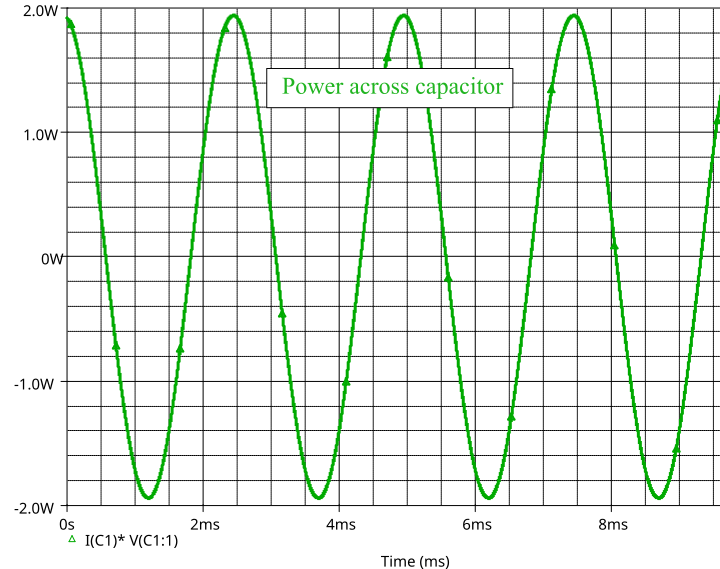
\includegraphics[width=\linewidth,height=0.4\textheight,keepaspectratio]{graph_task6d_power.png}
		\caption{Instantaneous capacitor power for Task 6d with the
			transient eliminated: the power alternates between positive
			and negative values as the capacitor stores and returns energy.}
		\label{fig:task6dpower}
	\end{figure}
	
	Fig.~\ref{fig:task6dpower} shows the same alternating
	storage-and-return pattern at this transient-free operating point.
	
	% =====================================================================
	\section{Discussion}
	\label{sec:discussion}
	The simulated responses agree with first-order RC theory within
	$0.3\,\%$ for the reported comparisons.  Since the simulator solves
	the same circuit equations, this agreement validates the analysis
	and measurement procedure rather than independently testing the
	underlying physics.
	
	Finite switch off-resistance explains the main switching deviations,
	through the pedestal of Eq.~\eqref{eq:pedestal}.  Leakage leaves
	discharge offsets of \SI{17.97}{\milli\volt}
	(Tasks 1/2) and \SI{39.92}{\milli\volt} (Task 6a), causing crossing
	measurements to overestimate the time constant.  Accounting for
	these offsets reduces the error below $0.15\,\%$.  The same leakage
	causes hold-interval droops of \SI{10}{\milli\volt} and
	\SI{4}{\milli\volt}, respectively.  The small sinusoidal residuals
	in Tasks 5 and 6d instead reflect initial-voltage mismatch and
	numerical integration: the reported deviations are
	\SI{3.1}{\milli\volt} and \SI{0.6}{\milli\volt}.
	
	The parameter variations confirm that $RC$ sets the transient time
	scale, while $\symup{T}_{\mathit{on}}/\tau$ controls pulse settling and $\omega\tau$
	controls sinusoidal attenuation and phase lag.  Task 6b preserves
	$\symup{T}_{\mathit{on}}/\tau=5$, retaining the nearly full-swing pulse response.
	Increasing $\omega\tau$ from $0.63$ in Task 4 to $2\pi$ in Task 6c
	reduces the transmitted amplitude from approximately $85\,\%$ to
	$16\,\%$ and increases the lag toward $90^\circ$.
	The steady-state capacitor power averages to zero, as illustrated
	in Figs.~\ref{fig:task4power} and \ref{fig:task6dpower}.
	
	Pre-charging to $\symup{V}_{0}=\symup{v}_{\mathit{C,SS}}(0)$ suppresses the switching
	transient, with the required charge determined by Eq.~\eqref{eq:q0}.
	Together, the results illustrate RC timing, filtering, and startup
	transient control.  Physical circuits would also exhibit capacitor
	leakage, equivalent series resistance, and switch-contact effects
	not included in the ideal component models.
	
	% =====================================================================
	\section{Reference}
	% =====================================================================
	% thebibliography normally typesets its own "\refname" heading
	% (\section*{References}) on top of the manual "1.9 Reference"
	% heading above, producing a duplicate title. Locally no-op the
	% starred \section call for just this one environment so only the
	% numbered heading remains.
	\begingroup
	\makeatletter
	\def\section{\@ifstar{\@gobble}{\@gobbletwo}}%
	\makeatother
	\begin{thebibliography}{9}
		\itemsep4pt
		
		\bibitem{sadiku}
		C. K. Alexander and M. N. O. Sadiku, \textit{Fundamentals of
			Electric Circuits}, 5th ed. New York, NY, USA: McGraw-Hill, 2013.
		
		\bibitem{boylestad}
		R. L. Boylestad, \textit{Introductory Circuit Analysis}, 11th ed.
		Upper Saddle River, NJ, USA: Pearson Prentice Hall, 2007.
		
		
	\end{thebibliography}
	\endgroup
	
\end{document}